%
% Template Laporan Skripsi/Thesis Universitas Indonesia
%
% @author  Ichlasul Affan, Azhar Kurnia
% @version 2.1.2
%
% Dokumen ini dibuat berdasarkan standar IEEE dalam membuat class untuk
% LaTeX dan konfigurasi LaTeX yang digunakan Fahrurrozi Rahman ketika
% membuat laporan skripsi, yang kemudian diadaptasi oleh Andreas Febrian dan
% Lia Sadita untuk template skripsi tahun 2010.
% Konfigurasi template sebelumnya telah disesuaikan dengan
% aturan penulisan thesis yang dikeluarkan UI pada tahun 2017.
%

%
% Tipe dokumen adalah report dengan satu kolom.
%
\documentclass[12pt, a4paper, onecolumn, twoside, final]{report}
\raggedbottom

% Load konfigurasi LaTeX untuk tipe laporan thesis
\usepackage{_internals/uithesis}
%


% Load konfigurasi khusus untuk laporan yang sedang dibuat
%-----------------------------------------------------------------------------%
% Informasi Mengenai Dokumen
%-----------------------------------------------------------------------------%
%
% Judul laporan.
\var{\judul}{Judul Karya Ilmiah Anda}
%
% Tulis kembali judul laporan, kali ini akan diubah menjadi huruf kapital
\Var{\Judul}{Judul Karya Ilmiah Anda}
%
% Tulis kembali judul laporan namun dengan bahasa Ingris
\var{\judulInggris}{Your Scientific Publication Title}

%
% Tipe laporan, dapat berisi Skripsi, Tugas Akhir, Thesis, atau Disertasi
\var{\type}{Skripsi}
%
% Tulis kembali tipe laporan, kali ini akan diubah menjadi huruf kapital
\Var{\Type}{Skripsi}
%
% Tulis nama penulis
\var{\penulis}{Nama Lengkap Anda}
%
% Tulis kembali nama penulis, kali ini akan diubah menjadi huruf kapital
\Var{\Penulis}{Nama Lengkap Anda}
%
% Tulis NPM penulis
\var{\npm}{Nomor Anda}
%
% Tuliskan Fakultas dimana penulis berada
\Var{\Fakultas}{Fakultas Anda}
\var{\fakultas}{Fakultas Anda}
%
% Tuliskan Program Studi yang diambil penulis
\Var{\Program}{Jurusan Anda}
\var{\program}{Jurusan Anda}
% Program Studi dalam bahasa inggris
\var{\studyProgram}{Your study program}
%
% Tuliskan tahun publikasi laporan
\Var{\bulanTahun}{Bulan Tahun}
%
% Tuliskan gelar yang akan diperoleh dengan menyerahkan laporan ini
\var{\gelar}{Gelar Jurusan Anda}
%
% Tuliskan tanggal pengesahan laporan, waktu dimana laporan diserahkan ke
% penguji/sekretariat
\var{\tanggalSiapSidang}{Tanggal Bulan Tahun}
%
% Tuliskan tanggal keputusan sidang dikeluarkan dan penulis dinyatakan
% lulus/tidak lulus
\var{\tanggalLulus}{Tanggal Bulan Tahun}
% Tuliskan tanggal pengesahan laporan final, waktu dimana laporan
% diserahkan ke perpustakaan
\var{\tanggalFinal}{Tanggal Bulan Tahun}
%
% Tuliskan pembimbing
\var{\pembimbingSatu}{Pembimbing Pertama Anda}
\var{\pembimbingDua}{Pembimbing Kedua Anda}
%
% Tuliskan penguji
\var{\pengujiSatu}{Penguji Pertama Anda}
\var{\pengujiDua}{Penguji Kedua Anda}

%-----------------------------------------------------------------------------%
% Judul Setiap Bab
%-----------------------------------------------------------------------------%
%
% Berikut ada judul-judul setiap bab.
% Silahkan diubah sesuai dengan kebutuhan.
%
\Var{\kataPengantar}{Kata Pengantar}
\Var{\babSatu}{Pendahuluan}
\Var{\babDua}{Kerangka Berpikir}
\Var{\babTiga}{Penggunaan Lanjutan}
\Var{\babEmpat}{Struktur Template}
\Var{\babLima}{Contoh Analisis dan Pembahasan}
\Var{\kesimpulan}{Penutup}

% Daftar pemenggalan suku kata dan istilah dalam LaTeX
%
% Hyphenation untuk Indonesia
%
% @author  Andreas Febrian
% @version 2.1.0
% @edit by Ichlasul Affan
%
% Tambahkan cara pemenggalan kata-kata yang salah dipenggal secara otomatis
% oleh LaTeX. Jika kata tersebut dapat dipenggal dengan benar, maka tidak
% perlu ditambahkan dalam berkas ini. Tanda pemenggalan kata menggunakan
% tanda '-'; contoh:
% menarik
%   --> pemenggalan: me-na-rik
%


% Silakan ganti ke bahasa Inggris (\selectlanguage{english}) jika Anda merasa terlalu banyak kata bahasa Inggris yang pemenggalannya tidak benar.
%\selectlanguage{english}


\hyphenation{
    % alphabhet A
    a-na-li-sa a-tur a-tur-an
    a-pli-ka-si
    % alphabhet B
    bab ba-ngun-an
    be-be-ra-pa
    ber-ge-rak
    ber-ke-lan-jut-an
    ber-o-per-ra-si
    ber-pe-nga-ruh
    % alphabhet C
    ca-ri Com-po-nent-UML
    % alphabhet D
    di-da-pat-kan di-sim-pan di-pim-pin di-tam-bah-kan di-tem-pat-kan de-ngan da-e-rah di-ba-ngun di-gu-na-kan da-pat di-nya-ta-kan
    di-se-mat-kan di-sim-bol-kan di-pi-lih di-li-hat de-fi-ni-si di-de-fi-ni-si-kan di-mo-del-kan di-mi-li-ki di-re-a-li-sa-si-kan di-su-sun
    % alphabhet E
    eks-pli-sit e-ner-gi en-gi-neer en-gi-neer-ing eks-klu-sif ele-men
    % alphabhet F
    fa-si-li-tas
    % alphabhet G
    ga-bung-an ge-rak ge-ne-ral ge-ne-ra-li-sa-si
    % alphabhet H
    ha-lang-an
    % alphabhet I
    in-fra-struk-tur i-ni-si-a-si
    % alphabhet J
    % alphabhet K
    ke-hi-lang-an
    ke-ter-hu-bung-an
    ku-ning
    kua-li-tas ka-me-ra ke-mung-kin-an ke-se-pa-ham-an
    % alphabhet L
    ling-kung-an
    % alphabhet M
    ma-na-je-men me-neng-ah meng-a-da-kan me-mo-ni-tor
    me-mer-lu-kan me-mo-del-kan men-de-fi-ni-si-kan meng-ak-ses me-ne-mu-kan
    meng-a-tas-i me-mo-di-fi-ka-si me-mung-kin-kan me-nge-na-i me-ngi-rim-kan meng-i-zin-kan
    meng-u-bah meng-a-dap-ta-si me-nya-ta-kan me-nyim-pan me-res-trik-si mi-cro-ser-vi-ce mi-cro-ser-vi-ces mo-di-fi-ka-si mo-dul mo-dule
    meng-a-tur meng-a-rah-kan mi-lik meng-gu-na-kan me-ne-ri-ma me-nga-la-mi
    % alphabhet N
    nya-ta non-eks-klu-sif
    % alphabhet O
    o-pe-ra-si or-ga-ni-sa-si
    % alphabhet P
	pe-nye-rap-an
	pe-ngon-trol
    pe-mo-del-an
    pe-ran  pe-ran-an-nya
    pem-ba-ngun-an pre-si-den pe-me-rin-tah pe-mi-li-han prio-ri-tas peng-am-bil-an
    peng-ga-bung-an pe-nga-was-an pe-ngem-bang-an
    pe-nga-ruh pe-nge-lo-la pa-ra-lel-is-me per-hi-tung-an per-ma-sa-lah-an
    pen-ca-ri-an pen-ce-ta-kan peng-struk-tur-an pen-ting pen-ting-nya pe-ngu-ku-ran
    pre-sen-ta-si
    % alphabhet Q
    % alphabhet R
    ran-cang-an re-fe-ren-si re-pre-sen-ta-si
    % alphabhet S
    sub-bab si-mu-la-si sa-ngat ska-la-bi-li-tas
    stan-dar-di-sa-si
    % alphabhet T
    te-ngah
    ter-da-pat
    trans-for-ma-si
    % alphabhet U
    % alphabhet V
    va-li-da-si va-ri-an va-ri-a-si va-ri-a-bi-li-tas ve-ri-fi-ka-si
    % alphabhet W
    % alphabhet X
    % alphabhet Y
    % alphabhet Z
    % special
}

% Daftar istilah yang mungkin perlu ditandai
%
% @author  Andreas Febrian
% @version 1.00
%
% Mendaftar seluruh istilah yang mungkin akan perlu dijadikan
% italic atau bold pada setiap kemunculannya dalam dokumen.
%

\var{\license}{\f{Creative Common License 1.0 Generic}}
\var{\bslash}{$\setminus$}


% Awal bagian penulisan laporan
\begin{document}
%
% Sampul Laporan
%
% Sampul Laporan

%
% @author  unknown
% @version 1.01
% @edit by Andreas Febrian
%

\begin{titlepage}
    \begin{center}
        \begin{figure}
            \begin{center}
                
\includegraphics[width=2.5cm]{assets/pics/makara_kuning.png}
            \end{center}
        \end{figure}
        \vspace*{0cm}
        \bo{
        	UNIVERSITAS INDONESIA\\
        }

        \vspace*{1.0cm}
        % judul thesis harus dalam 14pt Times New Roman
        \bo{\Judul} \\[1.0cm]

        \vspace*{2.5 cm}
        % harus dalam 14pt Times New Roman
        \bo{\Type}

        \vspace*{3 cm}
        % penulis dan npm
        \bo{\Penulis} \\
        \bo{\npm} \\

        \vspace*{5.0cm}

        % informasi mengenai fakultas dan program studi
        \bo{
        	FAKULTAS \Fakultas\\
        	PROGRAM STUDI \Program \\
        	DEPOK \\
        	\bulanTahun
        }
    \end{center}
\end{titlepage}

\forceclearchapter

%
% Gunakan penomeran romawi
\pagenumbering{roman}
%
% Menghilangkan penebalan pada huruf-huruf table of content
% dari halaman judul hingga daftar lampiran
\disableboldchapterintoc
%
% load halaman judul dalam
\addChapter{HALAMAN JUDUL}
%
% Halaman Judul Laporan
%
% @author  unknown
% @version 1.01
% @edit by Andreas Febrian
%

\begin{titlepage}
    \begin{center}\begin{figure}
            \begin{center}
                
\includegraphics[width=2.5cm]{assets/pics/makara.png}
            \end{center}
        \end{figure}
        \vspace*{0cm}
        \bo{
        	UNIVERSITAS INDONESIA\\
        }

        \vspace*{1.0cm}
        % judul thesis harus dalam 14pt Times New Roman
        \bo{\Judul} \\[1.0cm]

        \vspace*{2.5 cm}
        % harus dalam 14pt Times New Roman
        \bo{\Type} \\
        % keterangan prasyarat
        \bo{Diajukan sebagai salah satu syarat untuk memperoleh gelar \\
        \gelar}\\

        \vspace*{3 cm}
        % penulis dan npm
        \bo{\Penulis} \\
        \bo{\npm} \\

        \vspace*{5.0cm}

        % informasi mengenai fakultas dan program studi
        \bo{
        	FAKULTAS \Fakultas\\
        	PROGRAM STUDI \Program \\
        	DEPOK \\
        	\bulanTahun
        }
    \end{center}
\end{titlepage}

\forceclearchapter

%
% load halaman orisinalitas

% Menghilangkan penomoran
\pagenumbering{gobble}

\strcompare{Laporan Kerja Praktik}{\type}{}
{
	%
% Halaman Orisinalitas
%
% @author  Andreas Febrian
% @version 2.1.2
% @edit by Muhammad Aulia Adil Murtito
%

\chapter*{\uppercase{Halaman Pernyataan Orisinalitas}}
\thispagestyle{empty}
\vspace*{2cm}

% Untuk input gambar tanda tangan, silahkan sesuaikan xshift, yshift, dan width dengan gambar tanda tangan Anda
%\begin{tikzpicture}[remember picture,overlay,shift={(current page.north east)}]
%\node[anchor=north east,xshift=-8.5cm,yshift=-14.2cm]{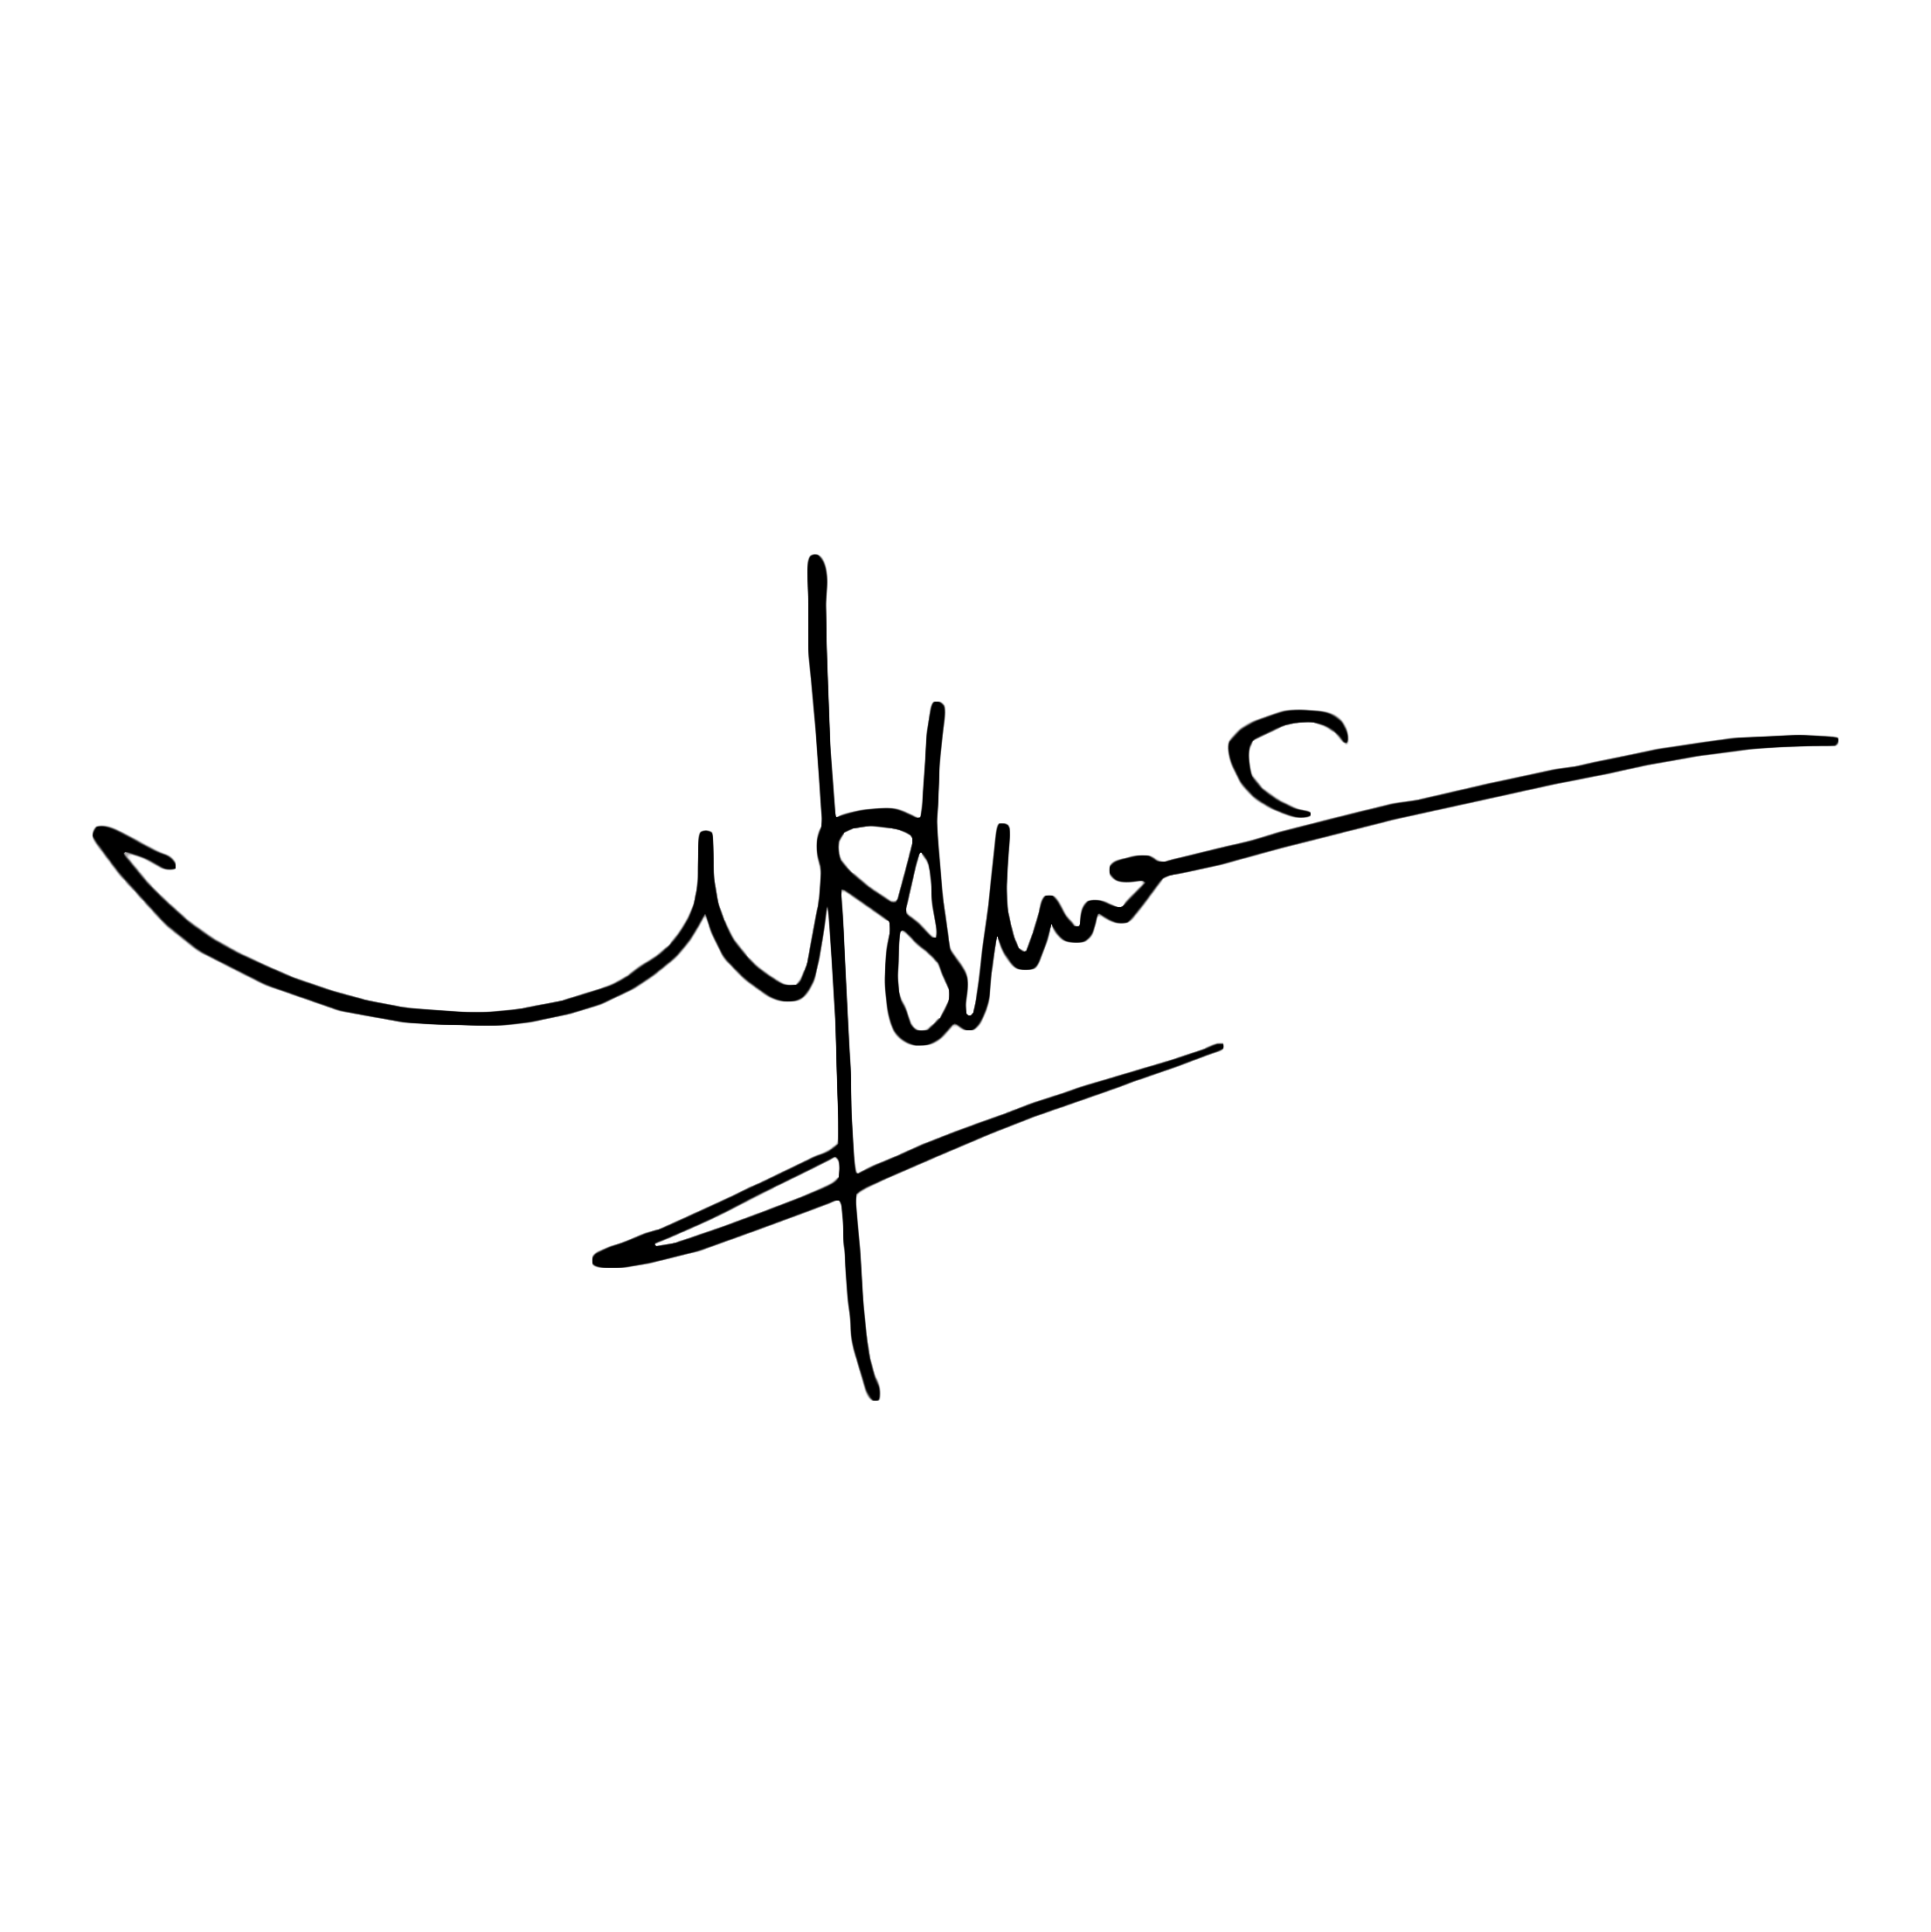
\includegraphics[width=3cm]{assets/pics/tanda_tangan_wikipedia.png}};
%\end{tikzpicture}

\begin{center}
	\bo{\type~ini adalah hasil karya saya sendiri, \\
	dan semua sumber baik yang dikutip maupun dirujuk \\
	telah saya nyatakan dengan benar.} \\
	\vspace*{2.6cm}

	\begin{tabular}{l c l}
	\bo{Nama} & : & \bo{\penulis} \\
	\bo{NPM} & : & \bo{\npm} \\
	\bo{Tanda Tangan} & : & \\
	& & \\
	& & \\
	\bo{Tanggal} & : & \bo{\tanggalSiapSidang} \\
	\end{tabular}
\end{center}

\newpage

	\forceclearchapter
}

% Memunculkan penomoran kembali
\pagenumbering{roman}

%
% setelah bagian ini, halaman dihitung sebagai halaman ke 2
\setcounter{page}{2}

%
% Lembar Penegesahan
\strcompare{Laporan Kerja Praktik}{\type}
{
	% Lembar Pengesahan Kerja Praktik dari LaTeX
	\addChapter{LEMBAR PERSETUJUAN DOSEN KERJA PRAKTIK}
	%
% Halaman Pengesahan Laporan Kerja Praktik
%
% @author  Andreas Febrian, Andre Tampubolon
% @version 2.1.2
% @edit by Ichlasul Affan
%

\chapter*{HALAMAN PERSETUJUAN DOSEN KERJA PRAKTIK}
\thispagestyle{empty}
\vspace*{0.4cm}
\noindent

\noindent
\begin{tabular}{ll p{9cm}}
	\multicolumn{3}{l}{\type~ini diajukan oleh:}  \\
	Nama&: & \penulis \\
	NPM&: & \npm \\
	Program Studi&: & \program \\
	Judul Kerja Praktik&: & \judul \\
\end{tabular} \\

\vspace*{1.0cm}

\noindent \bo{Telah berhasil diselesaikan laporan kerja praktik untuk
Fakultas \fakultas~dan dipresentasikan hasil kerja praktiknya sebagai
persyaratan yang harus dipenuhi dalam mata kuliah Kerja Praktik.}\\[0.2cm]

\begin{center}
	DOSEN MATA KULIAH KERJA PRAKTIK\\[2cm]
\end{center}

\begin{center}
	\underline{\pembimbingSatu}\\[0.1cm]
\end{center}

\vspace*{2.0cm}

\begin{tabular}{ll l}
	Ditetapkan di&: & Depok\\
	Tanggal&: & \tanggalLulus \\
\end{tabular}

\newpage

	\forceclearchapter
}
{
	\addChapter{LEMBAR PENGESAHAN}
	% Gunakan salah satu (comment atau hapus kode yang tidak perlu):
	% Lembar Pengesahan Tugas Akhir dari LaTeX
	\strcompare{Doktor}{\jenjang}
	{%
% Halaman Pengesahan Sidang (S3)
%
% @author  Andreas Febrian, Andre Tampubolon
% @version 2.1.2
% @edit by Ichlasul Affan
%

\chapter*{HALAMAN PENGESAHAN}
\thispagestyle{empty}
\vspace*{0.4cm}
\noindent

\noindent
\begin{tabular}{ll p{9cm}}
	\type~ini diajukan oleh&: & \\
	Nama&: & \penulis \\
	NPM&: & \npm \\
	Program Studi&: & \program \\
	Judul \type&: & \judul \\
\end{tabular} \\

\vspace*{1.0cm}

\noindent \bo{Telah berhasil dipertahankan di hadapan Dewan Penguji
dan diterima sebagai bagian persyaratan yang diperlukan untuk
memperoleh gelar Doktor pada Program Studi \program, Fakultas
\fakultas, Universitas Indonesia.}\\[0.2cm]

\begin{center}
	\bo{DEWAN PENGUJI}
\end{center}

\vspace*{0.3cm}

\def\blank{}
\begin{longtable}{l l p{7cm} l }
	\centering
	& & & \\
	Promotor&: & \pembimbingSatu & (\hspace*{3.0cm}) \\
	\ifx\blank\pembimbingDua
    \else
        & & & \\
    	Kopromotor&: & \pembimbingDua & (\hspace*{3.0cm}) \\
    \fi
    \ifx\blank\pembimbingTiga
    \else
        & & & \\
    	&: & \pembimbingTiga & (\hspace*{3.0cm}) \\
    \fi
	& & & \\
	Tim Penguji&: & \pengujiSatu~(Ketua) & (\hspace*{3.0cm}) \\
	& & & \\
	&: & \pengujiDua~(Anggota) & (\hspace*{3.0cm}) \\
	\ifx\blank\pengujiTiga
    \else
        & & & \\
    	&: & \pengujiTiga~(Anggota) & (\hspace*{3.0cm}) \\
    \fi
	\ifx\blank\pengujiEmpat
	\else
		& & & \\
		&: & \pengujiEmpat~(Anggota) & (\hspace*{3.0cm}) \\
	\fi
	\ifx\blank\pengujiLima
	\else
		& & & \\
		&: & \pengujiLima~(Anggota) & (\hspace*{3.0cm}) \\
	\fi
	\ifx\blank\pengujiEnam
	\else
		& & & \\
		&: & \pengujiEnam~(Anggota) & (\hspace*{3.0cm}) \\
	\fi
\end{longtable}

\vspace*{2.0cm}

\begin{tabular}{ll l}
	Ditetapkan di&: & Depok\\
	Tanggal&: & \tanggalLulus \\
\end{tabular}


\newpage
}
	{%
% Halaman Pengesahan Sidang
%
% @author  Andreas Febrian, Andre Tampubolon
% @version 2.1.2
% @edit by Muhammad Aulia Adil Murtito
%

\chapter*{HALAMAN PENGESAHAN}
\thispagestyle{empty}
\vspace*{0.4cm}
\noindent

\noindent
\begin{tabular}{ll p{9cm}}
	\type~ini diajukan oleh&: & \\
	Nama&: & \penulis \\
	NPM&: & \npm \\
	Program Studi&: & \program \\
	Judul \type&: & \judul \\
\end{tabular} \\

\vspace*{1.0cm}

\noindent \bo{Telah berhasil dipertahankan di hadapan Dewan Penguji
dan diterima sebagai bagian persyaratan yang diperlukan untuk
memperoleh gelar \jenjang~pada Program Studi \program, Fakultas
\fakultas, Universitas Indonesia.}\\[0.2cm]

\begin{center}
	\bo{DEWAN PENGUJI}
\end{center}

\vspace*{0.3cm}

\def\blank{}
\begin{tabular}{l l p{7cm} l }
	\centering
	& & & \\
	Pembimbing 1&: & \pembimbingSatu & (\hspace*{3.0cm}) \\
	\ifx\blank\pembimbingDua
    \else
        & & & \\
    	Pembimbing 2&: & \pembimbingDua & (\hspace*{3.0cm}) \\
    \fi
	& & & \\
	Penguji 1&: & \pengujiSatu & (\hspace*{3.0cm}) \\
	& & & \\
	Penguji 2&: & \pengujiDua & (\hspace*{3.0cm}) \\
	\ifx\blank\pengujiTiga
    \else
        & & & \\
    	Penguji 3&: & \pengujiTiga & (\hspace*{3.0cm}) \\
    \fi
\end{tabular}\\

\vspace*{2.0cm}

\begin{tabular}{ll l}
	Ditetapkan di&: & Depok\\
	Tanggal&: & \tanggalLulus \\
\end{tabular}


\newpage
}
	\forceclearchapter
	% Lembar Pengesahan dari PDF lain (misal: generated oleh SISIDANG [Fasilkom])
	%\putpdf{assets/pdfs/pengesahanSidang.pdf}
}


\strcompare{Laporan Kerja Praktik}{\type}{}
{
	%
	% Kata Pengantar
	\addChapter{\kataPengantar}
	%-----------------------------------------------------------------------------%
\chapter*{\kataPengantar}
%-----------------------------------------------------------------------------%
\pagestyle{first-pages}

Template ini disediakan untuk orang-orang yang berencana menggunakan \latex~untuk membuat dokumen tugas akhir.

\todo{Silakan ganti pesan ini dengan pendahuluan kata pengantar Anda.}

Ucapan Terima Kasih:
\begin{enumerate}[topsep=0pt,itemsep=-1ex,partopsep=1ex,parsep=1ex]
	\item Pembimbing.
	\item Dosen.
	\item Instansi.
	\item Orang tua.
	\item Sahabat.
	\item Teman.
\end{enumerate}

Penulis menyadari bahwa laporan \type~ini masih jauh dari sempurna. Oleh karena itu, apabila terdapat kesalahan atau kekurangan dalam laporan ini, Penulis memohon agar kritik dan saran bisa disampaikan langsung melalui \f{e-mail} \code{emailanda@mail.id}.

\begin{figure}
	\centering
	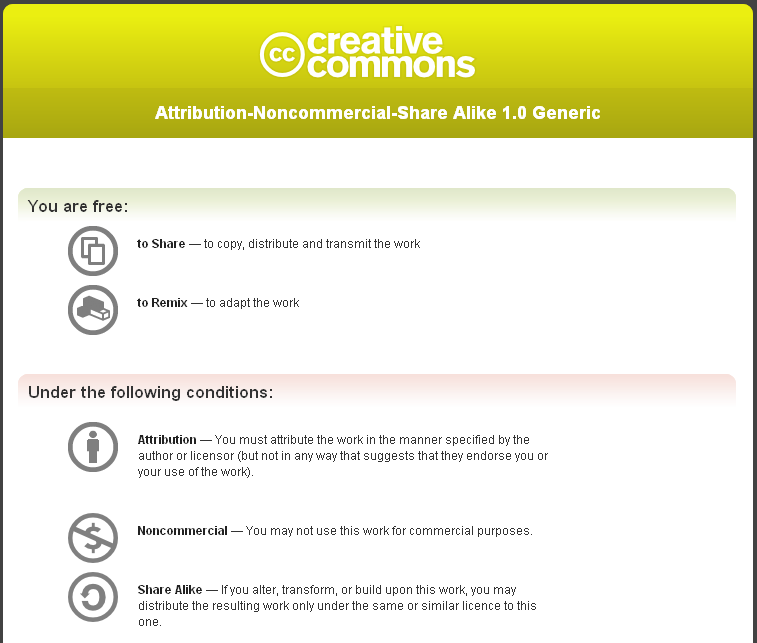
\includegraphics[width=0.74\textwidth]
	{assets/pics/creative_commons.png}
	\caption*{\license}
	\label{fig:lisensi}
\end{figure}

Terkait template ini, gambar lisensi di atas diambil dari \url{http://creativecommons.org/licenses/by-nc-sa/1.0/deed.en_CA}. Jika ingin mengentahui lebih lengkap mengenai \license, silahkan buka \url{http://creativecommons.org/licenses/by-nc-sa/1.0/legalcode}.
Seluruh dokumen yang dibuat dengan menggunakan template ini sepenuhnya menjadi hak milik pembuat dokumen dan bebas didistribusikan sesuai dengan keperluan masing-masing.
Lisensi hanya berlaku jika ada orang yang membuat template baru dengan menggunakan template ini sebagai dasarnya.

Penyusun template ingin berterima kasih kepada Andreas Febrian, Lia Sadita, Fahrurrozi Rahman, Andre Tampubolon, dan Erik Dominikus atas kontribusinya dalam template yang menjadi pendahulu template ini.
Penyusun template juga ingin mengucapkan terima kasih kepada Azhar Kurnia atas kontribusinya dalam template yang menjadi pendahulu template ini.

Semoga template ini dapat membantu orang-orang yang ingin mencoba menggunakan \latex.
Semoga template ini juga tidak berhenti disini dengan ada kontribusi dari para penggunanya.
Jika Anda memiliki perubahan yang dirasa penting untuk disertakan dalam template, silakan lakukan \f{fork} repositori Git template ini di \url{https://gitlab.com/ichlaffterlalu/latex-skripsi-ui-2017}, lalu lakukan \f{merge request} perubahan Anda terhadap \f{branch} \code{master}.
Kami berharap agar \f{template} ini dapat terus diperbarui mengikuti perubahan ketentuan dari pihak Rektorat Universitas Indonesia, dan hal itu tidak mungkin terjadi tanpa kontribusi dari teman-teman sekalian.

% Untuk input gambar tanda tangan, silahkan sesuaikan xshift, yshift, dan width dengan gambar tanda tangan Anda
%\begin{tikzpicture}[remember picture,overlay,shift={(current page.north east)}]
%\node[anchor=north east,xshift=-3cm,yshift=-6.2cm]{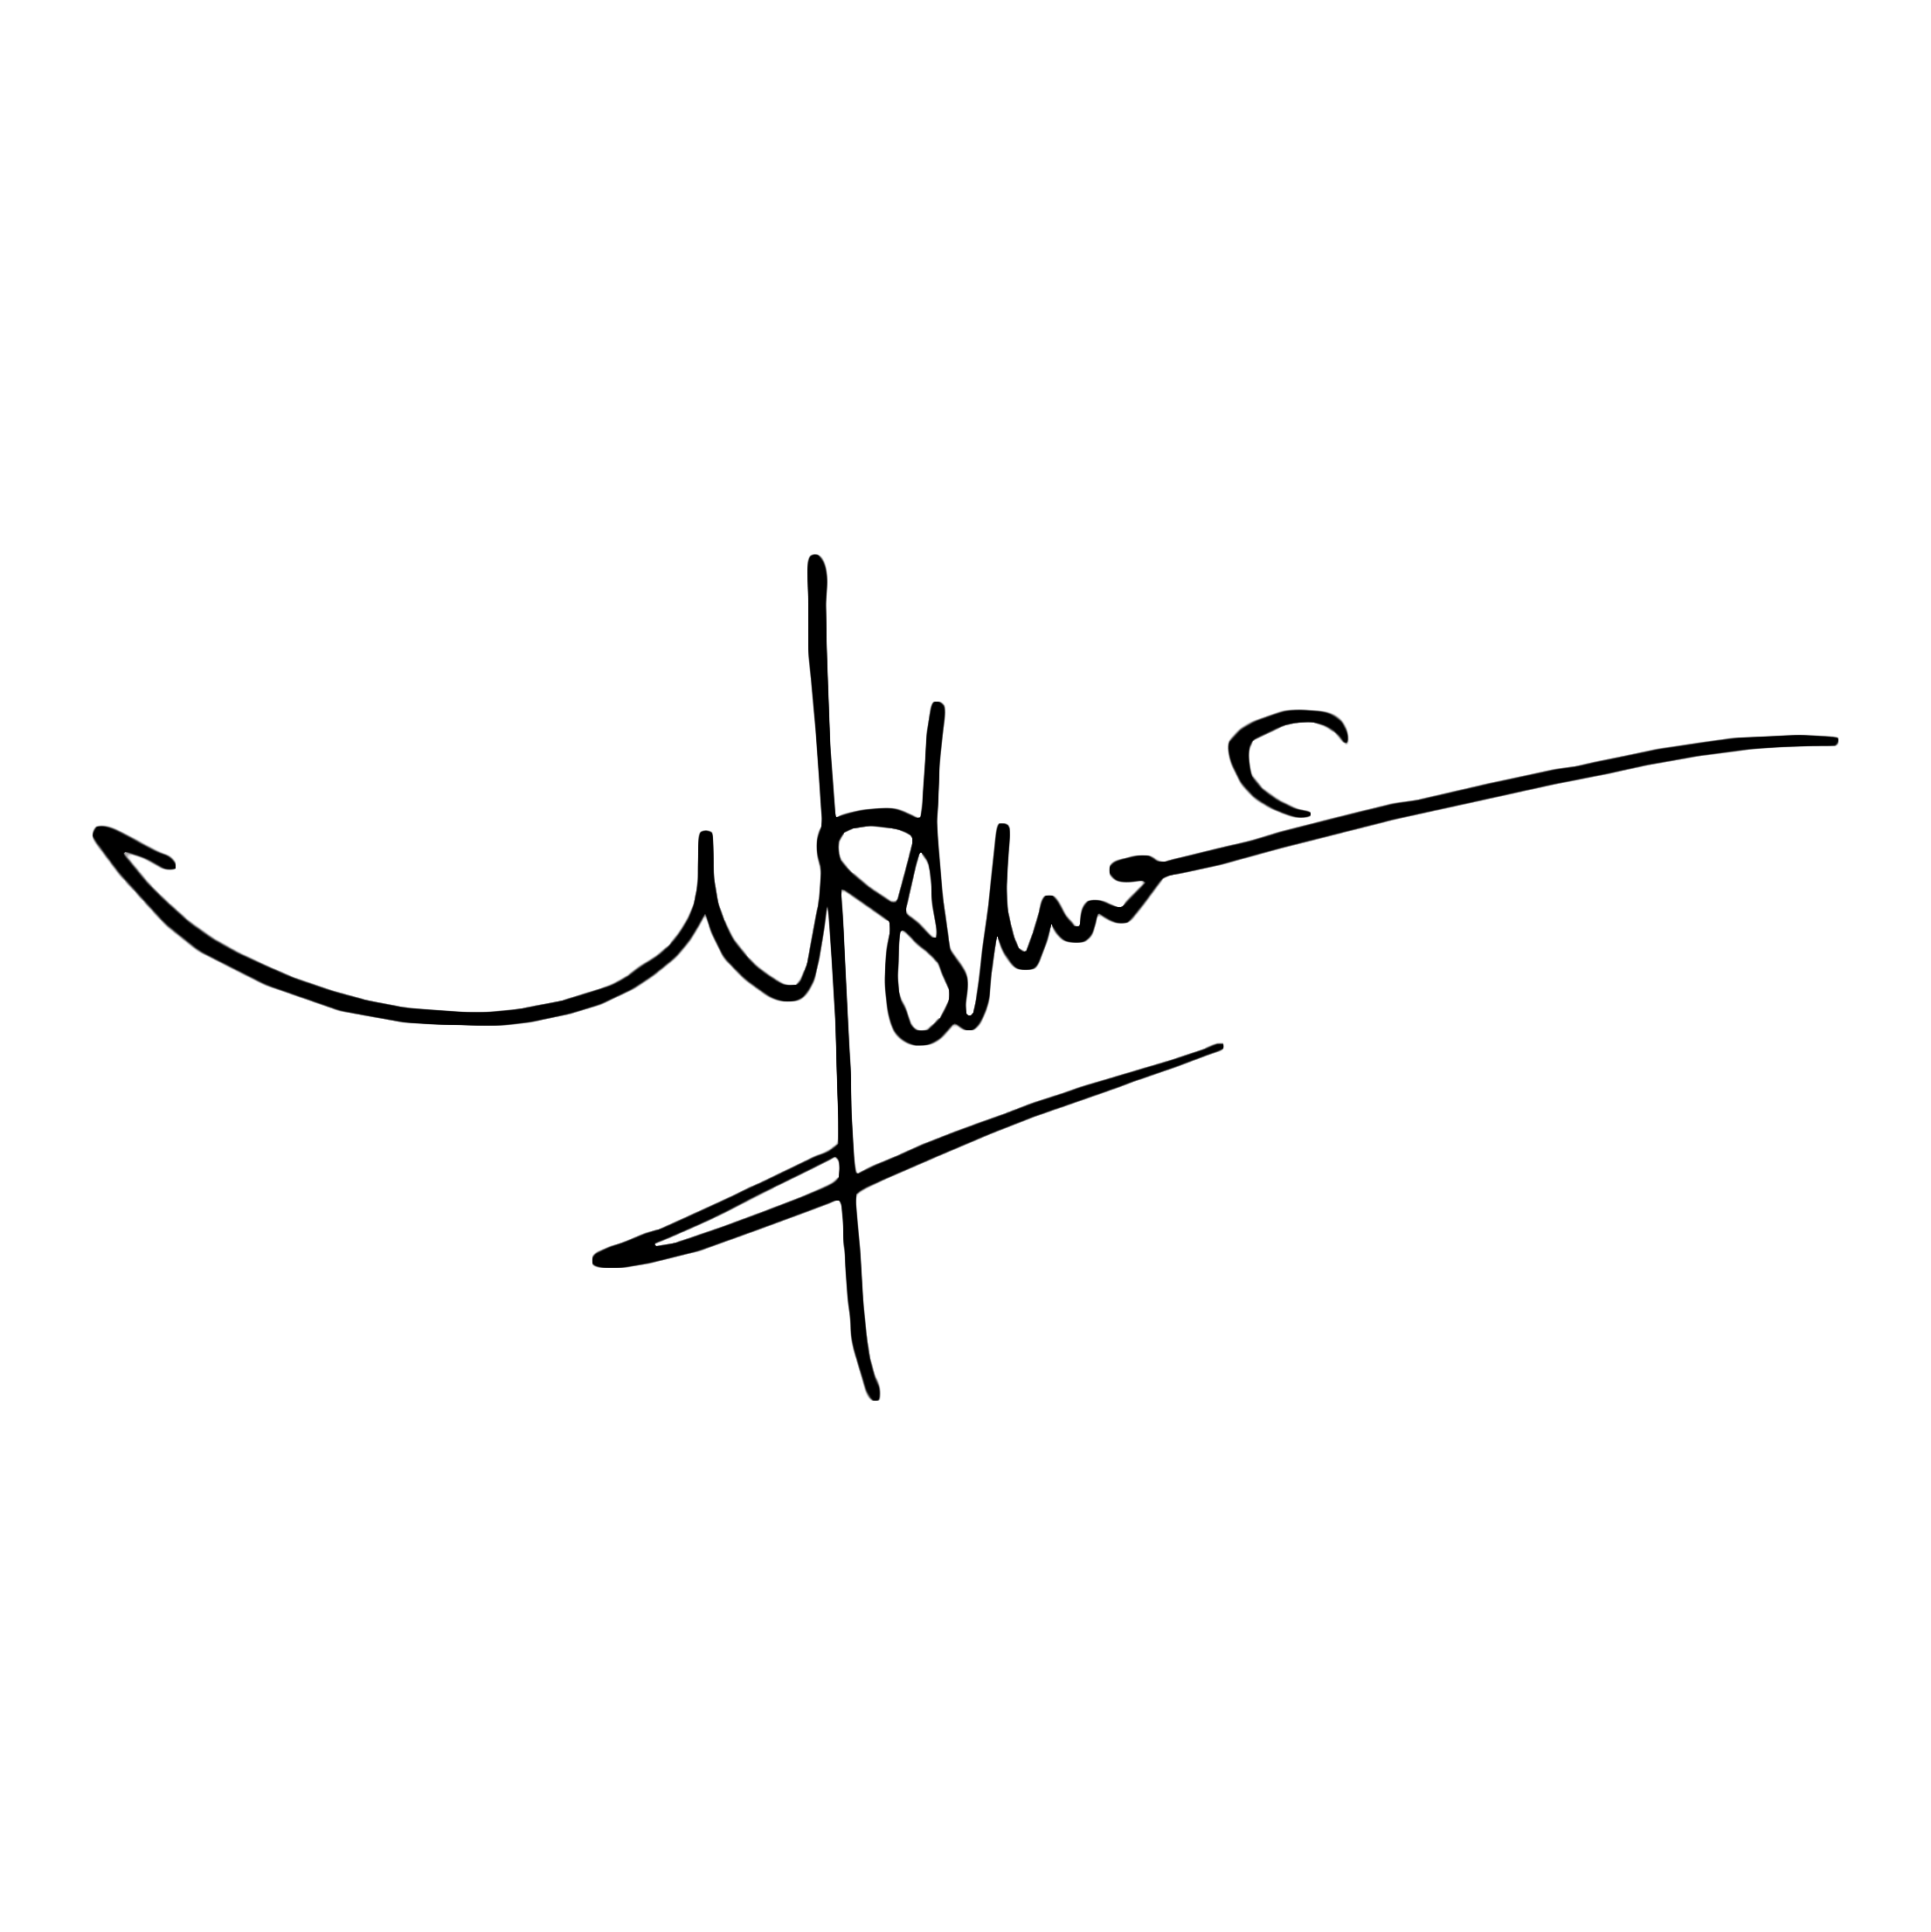
\includegraphics[width=3cm]{assets/pics/tanda_tangan_wikipedia.png}};
%\end{tikzpicture}

\vspace*{0.1cm}
\begin{flushright}
Depok, \tanggalSiapSidang\\[0.1cm]
\vspace*{1.5cm}
\penulis

\end{flushright}

	\forceclearchapter
	%
	% Lembar Persetujuan Publikasi Ilmiah
	\addChapter{LEMBAR PERSETUJUAN PUBLIKASI ILMIAH}
	%
% @author  Andre Tampubolon, Andreas Febrian
% @version 2.1.2
% @edit by Muhammad Aulia Adil Murtito
%

\chapter*{\uppercase{Halaman Pernyataan Persetujuan Publikasi Tugas Akhir untuk Kepentingan Akademis}}
\thispagestyle{empty}
\vspace*{0.2cm}
\noindent
Sebagai sivitas akademik Universitas Indonesia, saya yang bertanda
tangan di bawah ini:
\vspace*{0.4cm}


\begin{tabular}{p{4.2cm} l p{6cm}}
	\bo{Nama} & : & \penulis \\
	\bo{NPM} & : & \npm \\
	\bo{Program Studi} & : & \program\\
	\bo{Fakultas} & : & \fakultas\\
	\bo{Jenis Karya} & : & \type \\
\end{tabular}

\vspace*{0.6cm}
\noindent demi pengembangan ilmu pengetahuan, menyetujui untuk memberikan
kepada Universitas Indonesia \bo{Hak Bebas Royalti Noneksklusif
(\textit{Non-exclusive Royalty Free Right})} atas karya ilmiah saya yang berjudul:
\begin{center}
	\judul
\end{center}
beserta perangkat yang ada (jika diperlukan). Dengan Hak Bebas Royalti
Noneksklusif ini Universitas Indonesia berhak menyimpan,
mengalihmedia/formatkan, mengelola dalam bentuk pangkalan data
(\textit{database}), merawat, dan memublikasikan tugas akhir saya selama
tetap mencantumkan nama saya sebagai penulis/pencipta dan sebagai
pemilik Hak Cipta. \\

\noindent Demikian pernyataan ini saya buat dengan sebenarnya.

% Untuk input gambar tanda tangan, silahkan sesuaikan xshift, yshift, dan width dengan gambar tanda tangan Anda
%\begin{tikzpicture}[remember picture,overlay,shift={(current page.north east)}]
%\node[anchor=north east,xshift=-9cm,yshift=-23.5cm]{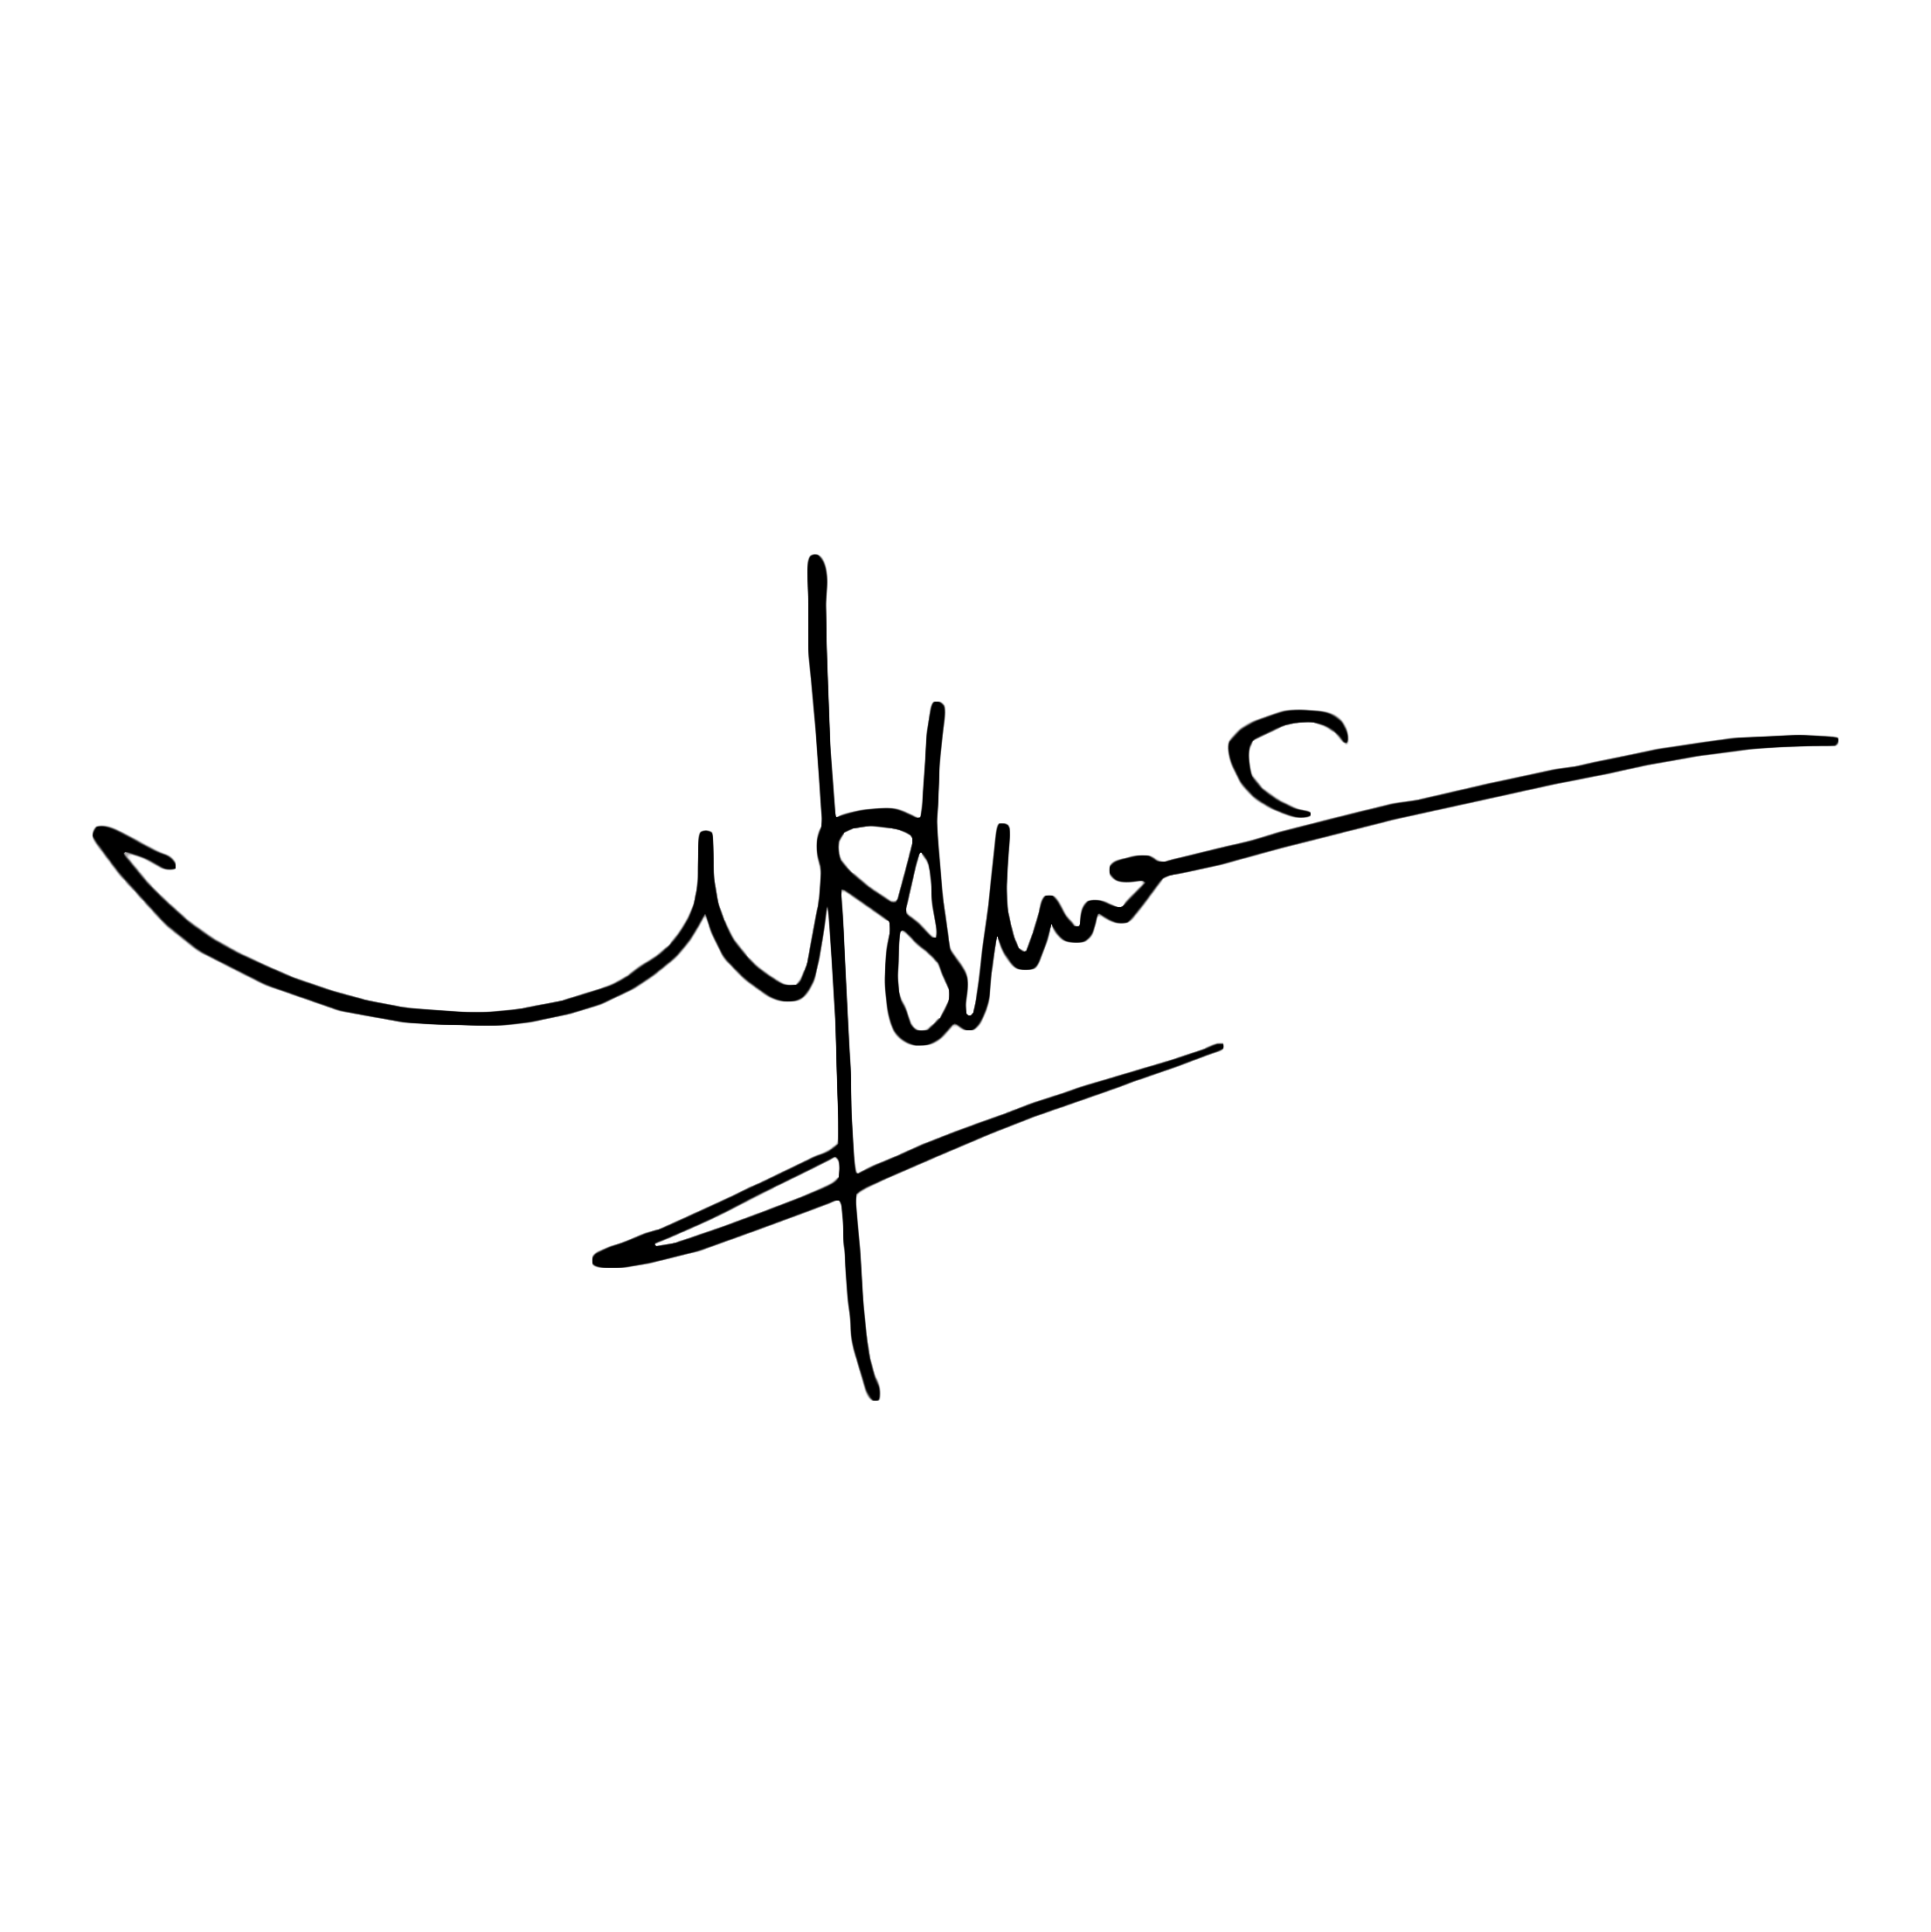
\includegraphics[width=3cm]{assets/pics/tanda_tangan_wikipedia.png}};
%\end{tikzpicture}

\begin{center}
	\vspace*{0.8cm}
	\begin{tabular}{lll}
		Dibuat di&: & Depok \\
		Pada tanggal&: & \tanggalSiapSidang \\
	\end{tabular}\\

	\vspace*{0.2cm}
	Yang menyatakan \\
	\vspace*{2cm}
	(\penulis)
\end{center}

\newpage

	\forceclearchapter
}

%
% Untuk halaman pertama setiap chapter mulai dari abstrak, tetap berikan mark universitas.
%
\pagestyle{first-pages}

%
\addChapter{ABSTRAK}
%
% Halaman Abstrak
%
% @author  Andreas Febrian
% @version 2.1.2
% @edit by Ichlasul Affan
%

\chapter*{Abstrak}
\singlespacing

\vspace*{0.2cm}

% Untuk conditional statement pembimbing dua
\def\blank{}

\noindent \begin{tabular}{l l p{10cm}}
	Nama&: & \penulis \\
	Program Studi&: & \program \\
	Judul&: & \judul \\
	Pembimbing&: & \pembimbingSatu \\
	\ifx\blank\pembimbingDua
    \else
        \ &\ & \pembimbingDua \\
    \fi
    \ifx\blank\pembimbingTiga
    \else
    	\ &\ & \pembimbingTiga \\
    \fi
\end{tabular} \\

\vspace*{0.5cm}

\noindent Isi abstrak. \\

\vspace*{0.2cm}

\noindent Kata kunci: \\ \f{Keyword} satu, kata kunci dua \\

\setstretch{1.4}
\newpage

%
%
%
% Halaman Abstract
%
% @author  Andreas Febrian
% @version 2.1.2
% @edit by Ichlasul Affan
%

\chapter*{ABSTRACT}
\singlespacing

\vspace*{0.2cm}

% Untuk conditional statement pembimbing dua
\def\blank{}

\noindent \begin{tabular}{l l p{11.0cm}}
	Name&: & \penulis \\
	Study Program&: & \studyProgram \\
	Title&: & \judulInggris \\
	Counsellor&: & \pembimbingSatu \\
	\ifx\blank\pembimbingDua
	\else
		\ &\ & \pembimbingDua \\
	\fi
	\ifx\blank\pembimbingTiga
	\else
		\ &\ & \pembimbingTiga \\
	\fi
\end{tabular} \\

\vspace*{0.5cm}

\noindent Abstract content. \\

\vspace*{0.2cm}

\noindent Key words: \\ Keyword one, keyword two \\

\setstretch{1.4}
\newpage


%
% Daftar isi, gambar, tabel, dan kode
%
\CAPinToC % All entries in ToC will be CAPITALIZED from here on
\phantomsection %hack to make them clickable
\singlespacing
\tableofcontents
\setstretch{1.4}
\clearpage
\phantomsection %hack to make them clickable
\singlespacing
\listoffigures
\setstretch{1.4}
\clearpage
\phantomsection %hack to make them clickable
\singlespacing
\listoftables
\setstretch{1.4}
\clearpage

%
% Daftar Kode Program
% Comment to disable.
%
\phantomsection %hack to make them clickable
\addcontentsline{toc}{chapter}{\lstlistlistingname}
\singlespacing
\listoflistings
\setstretch{1.4}
\clearpage

%
% Daftar Isi yang Didefinisikan Sendiri (Custom)
% Definisi jenis objek baru dapat dilakukan di uithesis.sty
% Uncomment to use.
%
%\phantomsection %hack to make them clickable
%\addcontentsline{toc}{chapter}{\listofthingname}
%\singlespacing
%\listofthing
%\setstretch{1.4}
%\clearpage

%
% Daftar Equation (Persamaan Matematis)
% Uncomment to use.
%
% \phantomsection %hack to make them clickable
% \addcontentsline{toc}{chapter}{\listofequname}
% \singlespacing
% \listofequ
% \setstretch{1.4}
% \clearpage

%
% Daftar Lampiran
% Comment to disable.
%
\phantomsection %hack to make them clickable
\addcontentsline{toc}{chapter}{\listofappendixname}
\singlespacing
\listofappendix
\setstretch{1.4}

% Table of content normal lagi hurufnya
\enableboldchapterintoc

\clearpage

% Jika penomoran romawi selesai di ganjil
%\naiveoddclearchapter
% Jika penomoran romawi selesai di genap
%\naiveevenclearchapter

\noCAPinToC % Revert to original \addcontentsline formatting

%
% Gunakan penomeran Arab (1, 2, 3, ...) setelah bagian ini.
%
\pagenumbering{arabic}
\pagestyle{standard}
% \setlength{\belowcaptionskip}{+2pt}


\setoddevenheader
%-----------------------------------------------------------------------------%
\chapter{\babSatu}
\label{bab:1}
%-----------------------------------------------------------------------------%
Pada bab ini, akan dijelaskan tentang latar belakang dan permasalahan yang diselesaikan pada penelitian ini.


%-----------------------------------------------------------------------------%
\section{Latar Belakang}
\label{sec:latarBelakang}
%-----------------------------------------------------------------------------%
\todo{Tentukan latar belakang dari penelitian Anda di sini (\f{background}).}

%-----------------------------------------------------------------------------%
\section{Permasalahan}
\label{sec:masalah}
%-----------------------------------------------------------------------------%
\todo{Sebutkan permasalahan penelitian Anda dari latar belakang tersebut.}

%-----------------------------------------------------------------------------%
\subsection{Definisi Permasalahan}
\label{sec:definisiMasalah}
%-----------------------------------------------------------------------------%
Berikut ini adalah rumusan permasalahan dari penelitian yang dilakukan:
\begin{itemize}
	\item Bagaimana cara membuat pertanyaan penelitian?
\end{itemize}
\todo{Tuliskan permasalahan yang ingin diselesaikan. Bisa juga berbentuk pertanyaan}


%-----------------------------------------------------------------------------%
\subsection{Batasan Permasalahan}
\label{sec:batasanMasalah}
%-----------------------------------------------------------------------------%
Berikut ini adalah asumsi yang digunakan sebagai batasan penelitian ini:
\begin{itemize}
	\item Salah satu batasannya adalah, ini hanya \f{template}.
\end{itemize}
\todo{Umumnya ada asumsi atau batasan yang digunakan untuk menjawab pertanyaan-pertanyaan penelitian diatas.}


%-----------------------------------------------------------------------------%
\section{Tujuan Penelitian}
\label{sec:tujuan}
%-----------------------------------------------------------------------------%
Berikut ini adalah tujuan penelitian yang dilakukan:
\begin{itemize}
	\item Untuk memberikan \f{template} yang dapat mempermudah skripsi orang lain.
\end{itemize}
\todo{Tuliskan tujuan penelitian Anda di bagian ini.}


%-----------------------------------------------------------------------------%
\section{Posisi Penelitian}
\label{sec:posisiPenelitian}
%-----------------------------------------------------------------------------%
\todo{Sebutkan posisi penelitian Anda. Ada baiknya jika Anda menggunakan gambar atau diagram. Template ini telah menyediakan contoh cara memasukkan gambar.}

\begin{figure}
	\centering
	
\includegraphics[width=0.4\textwidth]{assets/pics/makara.png}
	\caption{Penjelasan singkat terkait gambar.}
	\label{fig:research_position}
\end{figure}

\todo{Jelaskan \pic~\ref{fig:research_position} di sini.}


%-----------------------------------------------------------------------------%
\section{Langkah Penelitian}
\label{sec:langkahPenelitian}
%-----------------------------------------------------------------------------%
Berikut ini adalah langkah penelitian yang telah dilakukan:
\begin{enumerate}
	\item Tinjauan literatur \\
	Pada tahap ini, dipelajari teori-teori yang terkait dengan penelitian ini untuk mendapatkan konsep dasar yang dibutuhkan dalam mencapai tujuan penelitian.
	\item Analisis implementasi dan kesimpulan \\
	Pada tahap ini, digunakan studi kasus untuk analisis terkait kegunaan \f{template}. Setelah melakukan analisis tersebut, ditarik kesimpulan keseluruhan dari penelitian ini.
\end{enumerate}


%-----------------------------------------------------------------------------%
\section{Sistematika Penulisan}
\label{sec:sistematikaPenulisan}
%-----------------------------------------------------------------------------%
Sistematika penulisan laporan adalah sebagai berikut:
\begin{itemize}
	\item Bab 1 \babSatu \\
	    Bab ini mencakup latar belakang, cakupan penelitian, dan pendefinisian masalah.
	\item Bab 2 \babDua \\
	    Bab ini mencakup pemaparan terminologi dan teori yang terkait dengan penelitian berdasarkan hasil tinjauan pustaka yang telah digunakan, sekaligus memperlihatkan kaitan teori dengan penelitian.
	\item Bab 3 \babTiga \\
	    Apa itu Bab 3?
	\item Bab 4 \babEmpat \\
		Apa itu Bab 4?
	\item Bab 5 \babLima \\
	    Apa itu Bab 5?
	\item Bab 6 \kesimpulan \\
	    Bab ini mencakup kesimpulan akhir penelitian dan saran untuk pengembangan berikutnya.
\end{itemize}

\todo{Anda bisa mengubah atau menambahkan penjelasan singkat mengenai isi masing-masing bab. Setiap tugas akhir pasti ada yang berbeda pada bagian ini.}

\clearchapter
%-----------------------------------------------------------------------------%
\chapter{\babDua}
\label{bab:2}
%-----------------------------------------------------------------------------%
Untuk memulai penelitian, dibutuhkan kerangka berpikir yang sesuai untuk permasalahan yang ingin dipecahkan. Untuk membentuk kerangka berpikir yang sesuai, perlu dikaitkan dengan hasil studi literatur yang telah dilakukan. Oleh karena itu, pada bab ini, akan dijelaskan hasil studi literatur yang telah dilakukan yang telah dikaitan dengan kerangka kerja untuk penelitian ini.


%-----------------------------------------------------------------------------%
\section{Apa itu \latex?}
\label{sec:latex}
%-----------------------------------------------------------------------------%

%-----------------------------------------------------------------------------%
\subsection{\latex~Secara Singkat}
\label{sec:latexBrief}
%-----------------------------------------------------------------------------%
Berdasarkan \cite{latex:intro}: \\
\begin{tabular}{| p{13cm} |}
	\hline
	\\
	LaTeX is a family of programs designed to produce publication-quality typeset documents. It is particularly strong when working with mathematical symbols. \\
	The history of LaTeX begins with a program called TEX. In 1978, a computer scientist by the name of Donald Knuth grew frustrated with the mistakes that his publishers made in typesetting his work. He decided to create a typesetting program that everyone could easily use to typeset documents, particularly those that include formulae, and made it freely available. The result is TEX. \\
	Knuth's product is an immensely powerful program, but one that does focus very much on small details. A mathematician and computer scientist by the name of Leslie Lamport wrote a variant of TEX called  that focuses on document structure rather than such details. \\
	\\
	\hline
\end{tabular}

\vspace*{0.8cm}

Dokumen \latex~sangat mudah, seperti halnya membuat dokumen teks biasa.
Ada beberapa perintah yang diawali dengan tanda '\bslash'.
Seperti perintah \code{\bslash\bslash}~yang digunakan untuk memberi baris baru.
Perintah tersebut juga sama dengan perintah \code{\bslash{}newline}.
Pada bagian ini akan sedikit dijelaskan cara manipulasi teks dan perintah-perintah \latex~yang mungkin akan sering digunakan.
Jika ingin belajar hal-hal dasar mengenai \latex, silakan kunjungi:

\begin{itemize}
	\item \url{http://frodo.elon.edu/tutorial/tutorial/}, atau
	\item \url{http://www.maths.tcd.ie/~dwilkins/LaTeXPrimer/}
\end{itemize}


%-----------------------------------------------------------------------------%
\subsection{\latex~Kompiler dan IDE}
\label{sec:latexCompiler}
%-----------------------------------------------------------------------------%
Untuk menggunakan \latex~(pada konteks hanya sebagai pengguna), tidak perlu banyak tahu mengenai hal-hal didalamnya.
Dengan menggunakan \f{Integrated Development Environment} (IDE), penggunaan \latex~akan serupa dengan pembuatan dokumen secara visual, layaknya OpenOffice Writer atau Microsoft Word.
Orang-orang yang menggunakan \latex~relatif lebih teliti dan terstruktur mengenai cara penulisan yang dia gunakan, karena \latex~memaksa untuk seperti itu.

Untuk mencoba \latex, diperlukan kompiler dan IDE.
Bagi pengguna Microsoft Windows dan Mac OS, instalasi kompiler \latex~dapat menggunakan MikTeX (\url{https://miktex.org/download}).
Bagi pengguna Linux, instalasi kompiler \latex~dapat menggunakan Texlive ( \url{http://www.tug.org/texlive/}).
Distro-distro \f{mainstream} di Linux seperti Ubuntu biasanya telah menyediakan \f{package} \code{texlive} melalui \f{package manager}.
Apabila ingin melakukan instalasi Texlive melalui \f{package manager}, lakukan instalasi package \code{texlive-full} atau setidaknya \code{texlive-science} agar prasyarat \f{template} ini tersedia secara lengkap.

Beberapa text editor atau IDE yang dapat digunakan adalah sebagai berikut:
\begin{itemize}
	\item TeXstudio (\url{https://www.texstudio.org/}).
	\item TeXWorks (biasanya bawaan dari MikTeX).
	\item Texmaker (\url{http://www.xm1math.net/texmaker/}).
	\item Microsoft Visual Studio Code, dengan \f{plugin} LaTeX Workshop (\url{https://marketplace.visualstudio.com/items?itemName=James-Yu.latex-workshop}). Untuk menggunakan \f{plugin} tersebut, diperlukan instalasi MikTeX dan Perl. Alternatif lain untuk persyaratan tersebut adalah menggunakan \f{plugin} Remote - WSL jika memiliki distro Windows Subsystem for Linux (WSL) 2 yang sudah terpasang \code{texlive}.
\end{itemize}


%-----------------------------------------------------------------------------%
\section{Panduan Pengunaan Dasar \latex}
\label{sec:latexUsage}
%-----------------------------------------------------------------------------%

%-----------------------------------------------------------------------------%
\subsection{Bold, Italic, dan Underline}
\label{sec:latexBIU}
%-----------------------------------------------------------------------------%
Hal pertama yang mungkin ditanyakan adalah bagaimana membuat huruf tercetak tebal, miring, atau memiliki garis bawah.
Pada Texmaker, Anda bisa melakukan hal ini seperti halnya saat mengubah dokumen dengan OO Writer.
Namun jika tetap masih tertarik dengan cara lain, ini dia:

\begin{itemize}
	\item \bo{Bold} \\
	Gunakan perintah \code{\bslash{}textbf$\lbrace\rbrace$} atau
	\code{\bslash{}bo$\lbrace\rbrace$}.
	\item \f{Italic} \\
	Gunakan perintah \code{\bslash{}textit$\lbrace\rbrace$} atau
	\code{\bslash{}f$\lbrace\rbrace$}.
	\item \underline{Underline} \\
	Gunakan perintah \code{\bslash{}underline$\lbrace\rbrace$}.
	\item $\overline{Overline}$ \\
	Gunakan perintah \code{\bslash{}overline}.
	\item $^{superscript}$ \\
	Gunakan perintah \code{\bslash{}$\lbrace\rbrace$}.
	\item $_{subscript}$ \\
	Gunakan perintah \code{\bslash{}\_$\lbrace\rbrace$}.
\end{itemize}

Perintah \code{\bslash{}f} dan \code{\bslash{}bo} hanya dapat digunakan jika package \code{uithesis} digunakan.


%-----------------------------------------------------------------------------%
\subsection{Memasukan Gambar}
\label{sec:latexImage}
%-----------------------------------------------------------------------------%
Setiap gambar dapat diberikan caption dan diberikan label. Label dapat digunakan untuk menunjuk gambar tertentu.
Jika posisi gambar berubah, maka nomor gambar juga akan diubah secara
otomatis.
Begitu juga dengan seluruh referensi yang menunjuk pada gambar tersebut.
Contoh sederhana adalah \pic~\ref{fig:testGambar}.
Silahkan lihat code \latex~dengan nama bab2.tex untuk melihat kode lengkapnya.
Harap diingat bahwa caption untuk gambar selalu terletak dibawah gambar.

\begin{figure}
	\centering
	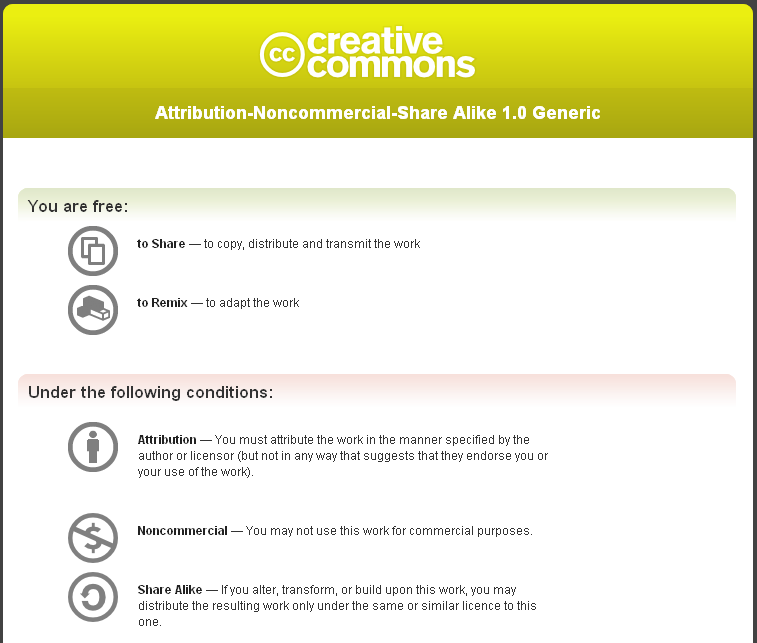
\includegraphics[width=0.50\textwidth]
	{assets/pics/creative_commons.png}
	\caption{\license.}
	\label{fig:testGambar}
\end{figure}


%-----------------------------------------------------------------------------%
\section{Membuat Tabel}
\label{sec:latexTable}
%-----------------------------------------------------------------------------%
Tabel pada Latex dapat dibuat dengan bantuan \textit{website} seperti \url{https://www.tablesgenerator.com/}. Dengan menggunakan \textit{website} ini, maka pembuatan tabel akan menjadi lebih mudah. \textit{User interface} dari \url{https://www.tablesgenerator.com/} dapat dilihat pada Gambar \ref{fig:tablesgenerator}.

\begin{figure}
	\centering
	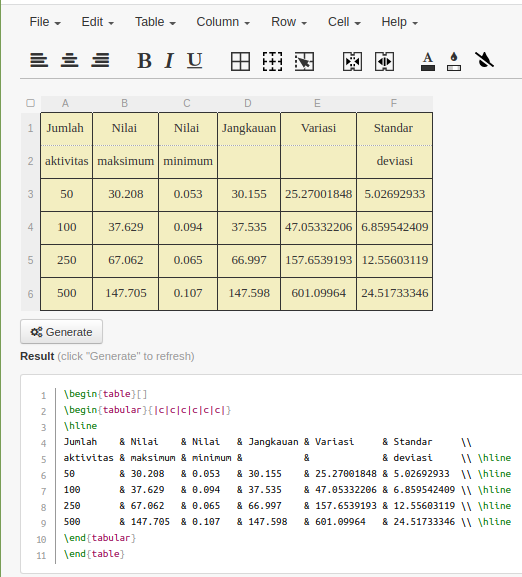
\includegraphics[width=0.5\textwidth]{assets/pics/tablesgenerator-dot-com.png}
	\caption{\textit{User interface} dari \textit{website} https://www.tablesgenerator.com/}
	\label{fig:tablesgenerator}
\end{figure}

Di sisi lain, tabel juga dapat diberi label dan caption seperti pada gambar.
Caption pada tabel terletak pada bagian atas tabel.
Contoh tabel sederhana dapat dilihat pada \tab~\ref{tab:tab1}.

\begin{table}
	\centering
	\caption{Contoh Tabel}
	\label{tab:tab1}
	\begin{tabular}{| l | c r |}
		\hline
		& kol 1 & kol 2 \\
		\hline
		baris 1 & 1 & 2 \\
		baris 2 & 3 & 4 \\
		baris 3 & 5 & 6 \\
		baris 4 & 7 & 8 \\
		baris 5 & 9 & 10 \\
		\hline
		jumlah  & 25 & 30 \\
		\hline
	\end{tabular}
\end{table}

Adapun untuk membuat tabel panjang yang bisa melebihi dari satu halaman, gunakan perintah \code{\bslash{}begin\{longtable\}} sebagai pengganti \code{\bslash{}begin\{table\}}. Di dalam \code{longtable} tidak perlu lagi ada \code{\bslash{}begin\{tabular\}}. Kemudian, tambahkan tanda \code{\bslash{}\bslash{}} setelah baris \code{\bslash{}label\{....\}}, agar tidak menimbulkan error saat menampilkan \f{caption} di bagian atas tabel. Kemudian, untuk membatasi header yang ingin diulang pada halaman-halaman berikutnya, gunakan perintah \code{\bslash{}endhead}. Contohnya adalah sebagai berikut:

\begin{longtable}{| l | c r |}
\caption{Contoh Tabel Panjang}
\label{tab:tab2} \\
\hline
& kol 1 & kol 2 \\
\hline
\endfirsthead % batas akhir header yang akan muncul di halaman pertama
\hline
& kol 1 & kol 2 \\
\hline
\endhead % batas akhir header yang akan muncul di halaman berikutnya
baris 1  & 1 & 2 \\
baris 2  & 3 & 4 \\
baris 3  & 5 & 6 \\
baris 4  & 7 & 8 \\
baris 5  & 9 & 10 \\
baris 6  & 11 & 12 \\
baris 7  & 13 & 14 \\
baris 8  & 15 & 16 \\
baris 9  & 17 & 18 \\
baris 10 & 19 & 20 \\
baris 11 & 21 & 22 \\
baris 12 & 23 & 24 \\
baris 13 & 25 & 26 \\
baris 14 & 27 & 28 \\
baris 15 & 29 & 30 \\
\hline
\end{longtable}

Ada jenis tabel lain yang dapat dibuat dengan \latex~berikut beberapa diantaranya.
Contoh-contoh ini bersumber dari \url{http://en.wikibooks.org/wiki/LaTeX/Tables}

\begin{table}
	\centering
	\caption{An Example of Rows Spanning Multiple Columns}
	\label{row.spanning}
	\begin{tabular}{|l|l|*{6}{c|}}
		\hline % create horizontal line
		No & Name & \multicolumn{3}{|c|}{Week 1} & \multicolumn{3}{|c|}{Week 2} \\
		\cline{3-8} % create line from 3rd column till 8th column
		& & A & B & C & A & B & C\\
		\hline
		1 & Lala & 1 & 2 & 3 & 4 & 5 & 6\\
		2 & Lili & 1 & 2 & 3 & 4 & 5 & 6\\
		3 & Lulu & 1 & 2 & 3 & 4 & 5 & 6\\
		\hline
	\end{tabular}
\end{table}

\begin{table}
	\centering
	\caption{An Example of Columns Spanning Multiple Rows}
	\label{column.spanning}
	\begin{tabular}{|l|c|l|}
		\hline
		Percobaan & Iterasi & Waktu \\
		\hline
		Pertama & 1 & 0.1 sec \\ \hline
		\multirow{2}{*}{Kedua} & 1 & 0.1 sec \\
		& 3 & 0.15 sec \\
		\hline
		\multirow{3}{*}{Ketiga} & 1 & 0.09 sec \\
		& 2 & 0.16 sec \\
		& 3 & 0.21 sec \\
		\hline
	\end{tabular}
\end{table}

\begin{table}
	\centering
	\caption{An Example of Spanning in Both Directions Simultaneously}
	\label{mix.spanning}
	\begin{tabular}{cc|c|c|c|c|}
		\cline{3-6}
		& & \multicolumn{4}{|c|}{Title} \\ \cline{3-6}
		& & A & B & C & D \\ \hline
		\multicolumn{1}{|c|}{\multirow{2}{*}{Type}} &
		\multicolumn{1}{|c|}{X} & 1 & 2 & 3 & 4\\ \cline{2-6}
		\multicolumn{1}{|c|}{}                        &
		\multicolumn{1}{|c|}{Y} & 0.5 & 1.0 & 1.5 & 2.0\\ \cline{1-6}
		\multicolumn{1}{|c|}{\multirow{2}{*}{Resource}} &
		\multicolumn{1}{|c|}{I} & 10 & 20 & 30 & 40\\ \cline{2-6}
		\multicolumn{1}{|c|}{}                        &
		\multicolumn{1}{|c|}{J} & 5 & 10 & 15 & 20\\ \cline{1-6}
	\end{tabular}
\end{table}


%-----------------------------------------------------------------------------%
\section{Keterkaitan Teori Dengan Penelitian}
\label{sec:keterkaitan}
%-----------------------------------------------------------------------------%
\todo{Ada baiknya setelah menjelaskan teori-teori, Anda menjelaskan apa kaitan teori tersebut dengan penelitian Anda. Hal ini tentunya membantu pembaca dalam memahami bahwa teori yang Anda paparkan memang penting untuk memahami penelitian Anda nantinya.}

\begin{figure}
	\centering
	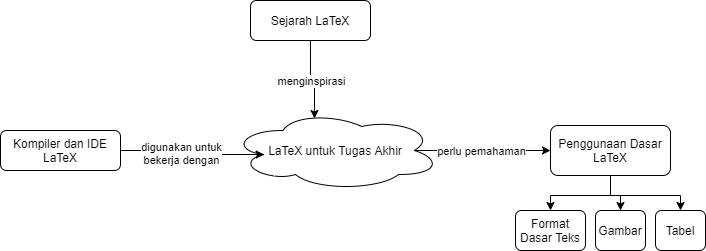
\includegraphics[width=\textwidth]{assets/pics/research_concept_map.png}
	\caption{Keterkaitan konsep hasil studi literatur terhadap penelitian}
	\label{fig:research_concept_map}
\end{figure}

\todo{Jelaskan \pic~\ref{fig:research_concept_map} di sini. Setiap gambar pada tugas akhir butuh penjelasan. Gambar hadir untuk mempermudah membaca memahami konteks, tetapi tidak bisa berdiri sendiri tanpa penjelasan. Terkait gambar, Anda juga bisa mengatur skalanya. Gambar kali ini lebarnya 0,8x dari lebar teks halaman.}

\clearchapter
%-----------------------------------------------------------------------------%
\chapter{\babTiga}
\label{bab:3}
%-----------------------------------------------------------------------------%
Bab ini menjelaskan tentang hal-hal \f{advanced} dalam \latex. Hal ini mencakup bagaimana cara menulis persamaan matematis di \latex, menambahkan daftar isi, catatan, PDF, menambahkan kode, bahkan menambahkan perintah baru.

\todo{Sejatinya bab ini digunakan untuk membahas inti dari penelitian Anda. Sesuaikan saja dengan kebutuhkan Anda: misalkan bab tiga Anda adalah penjelasan terkait desain sistem.}


%-----------------------------------------------------------------------------%
\section{Membuat Persamaan Matematis}
\label{sec:mathEqu}
%-----------------------------------------------------------------------------%
Di \latex, kita dapat membuat persamaan matematis baik yang terdiri dari satu persamaan maupun lebih dari satu persamaan. Anda bisa mencoba mengikuti dan memahami contoh kode yang ada di \f{template} ini untuk kebutuhan tugas akhir Anda. Menggunakan \latex~juga perlu latihan dan lihai memahami dokumentasi.

%-----------------------------------------------------------------------------%
\subsection{Satu Persamaan}
\label{sec:oneEqu}
%-----------------------------------------------------------------------------%

\noindent \begin{align}\label{equ:garis}
	\cfrac{y - y_{1}}{y_{2} - y_{1}} =
	\cfrac{x - x_{1}}{x_{2} - x_{1}}
\end{align}

\equ~\ref{equ:garis} diatas adalah persamaan garis.
\equ~\ref{equ:garis} dan \ref{equ:bola} sama-sama dibuat dengan perintah \code{\bslash{}align}.
Perintah ini juga dapat digunakan untuk menulis lebih dari satu persamaan.

\noindent \begin{align}\label{equ:bola}
	\underbrace{|\overline{ab}|}_{\text{pada bola $|\overline{ab}| = r$}}
	= \sqrt[2]{(x_{b} - x_{a})^{2} + (y_{b} - y_{a})^{2} +
		\vert\vert(z_{b} - z_{a})^{2}}
\end{align}

%-----------------------------------------------------------------------------%
\subsection{Lebih dari Satu Persamaan}
\label{sec:multiEqu}
%-----------------------------------------------------------------------------%
\noindent \begin{align}\label{equ:matriks}
	|\overline{a} * \overline{b}| &= |\overline{a}| |\overline{b}| \sin\theta
	\\[0.2cm]
	\overline{a} * \overline{b} &=
	\begin{array}{| c c c |}
		\hat{i} & x_{1} & x_{2} \\
		\hat{j} & y_{1} & y_{2} \\
		\hat{k} & z_{1} & z_{2} \\
	\end{array} \nonumber \\[0.2cm]
	&= \hat{i} \,
	\begin{array}{ | c c | }
		y_{1} & y_{2} \\
		z_{1} & z_{2} \\
	\end{array}
	+ \hat{j} \,
	\begin{array}{ | c c | }
		z_{1} & z_{2} \\
		x_{1} & x_{2} \\
	\end{array}
	+ \hat{k} \,
	\begin{array}{ | c c | }
		x_{1} & x_{2} \\
		y_{1} & y_{2} \\
	\end{array}
	\nonumber
\end{align}

Pada \equ~\ref{equ:matriks} dapat dilihat beberapa baris menjadi satu bagian
dari \equ~\ref{equ:matriks}.
Sedangkan dibawah ini dapat dilihat bahwa dengan cara yang sama, \equ~
\ref{equ:gabungan1}, \ref{equ:gabungan2}, dan \ref{equ:gabungan3} memiliki nomor
persamaannya masing-masing.

\noindent \begin{align}\label{equ:gabungan1}
	\int_{a}^{b} f(x)\, dx + \int_{b}^{c} f(x) \, dx = \int_{a}^{c} f(x) \, dx
	\\\label{equ:gabungan2}
	\lim_{x \to \infty} \frac{f(x)}{g(x)} = 0 \hspace{1cm}
	\text{jika pangkat $f(x)$ $<$ pangkat $g(x)$} \\\label{equ:gabungan3}
	a^{m^{a \, ^{n}\log b }} = b^{\frac{m}{n}}
\end{align}



%-----------------------------------------------------------------------------%
\section{Mengubah Tampilan Teks}
\label{sec:textFormatting}
%-----------------------------------------------------------------------------%
Beberapa perintah yang dapat digunakan untuk mengubah tampilan adalah:
\begin{itemize}
	\item \bslash{}f \\
	Merupakan alias untuk perintah \bslash textit, contoh
	\f{contoh hasil tulisan}.
	\item \bslash{}bi \\
	\bi{Contoh hasil tulisan}.
	\item \bslash{}bo \\
	\bo{Contoh hasil tulisan}.
	\item \bslash{}m \\
	\m{Contoh hasil tulisan}.
	\item \bslash{}mc \\
	\mc{Contoh hasil tulisan}.
	\item \bslash{}code \\
	\code{Contoh hasil tulisan}.
\end{itemize}


%-----------------------------------------------------------------------------%
\section{Menambahkan Kode Program}
\label{sec:codeListing}
% Hal baru di template 2017
%-----------------------------------------------------------------------------%
Pada \latex, kode program seringkali disebut \f{listing}. Kita bisa memasukkan kode program (\f{listing}) ke dalam tugas akhir kita seperti kode Java seperti berikut:
\lstinputlisting[language=Java, caption=Kode sampel Java, label=code:java]{assets/codes/3-sample.java}

\f{Syntax highlighting} kini sudah bisa dilakukan secara otomatis oleh \f{library} yang ada di \latex.
Sudah tidak perlu lagi membuat skrip manual untuk menambahkan \f{syntax highlighting} sendiri.
Cukup definisikan bahasa pemrograman yang digunakan, pada parameter \code{language=} di perintah \code{\bslash{}lstinputlisting}.

Berikut ini adalah daftar bahasa pemrograman yang didukung \f{library} \code{listings}: ABAP, ACSL, Ada, Algol, Ant, Assembler, Awk, bash, Basic, C\#, C++, C, Caml, Clean, Cobol, Comal, csh, Delphi, Eiffel, Elan, erlang, Euphoria, Fortran, GCL, Gnuplot, Haskell, HTML, IDL, inform, Java, JVMIS, ksh, Lisp, Logo, Lua, make, Mathematica, Matlab, Mercury, MetaPost, Miranda, Mizar, ML, Modelica, Modula-2, MuPAD, NASTRAN, Oberon-2, Objective C, OCL, Octave, Oz, Pascal, Perl, PHP, PL/I, Plasm, POV, Prolog, Promela, Python, R, Reduce, Rexx, RSL, Ruby, S, SAS, Scilab, sh, SHELXL, Simula, SQL, tcl, TeX, VBScript, Verilog, VHDL, VRML, XML, XSLT. \citep{latex:source_code_listings}

Satu contoh lagi, sebuah kode bahasa pemrograman Python:
\lstinputlisting[language=Python, caption=Kode sampel Python, label=code:python]{assets/codes/3-sample.py}

Anda juga bisa menambahkan \f{caption} untuk memberikan ringkasan tentang kode tersebut.
Namun, jangan lupa untuk menjelaskan kode melalui paragraf, terutama pada bagian-bagian yang perlu penjelasan lebih.
Penting bagi pembaca untuk memahami mengapa kode tersebut disertakan dalam laporan tugas akhir Anda.


%-----------------------------------------------------------------------------%
\section{Memberikan Catatan}
\label{sec:note}
%-----------------------------------------------------------------------------%
Ada dua perintah untuk memberikan catatan penulisan dalam dokumen yang Anda kerjakan, yaitu:
\begin{itemize}
	\item \code{\bslash{}todo} \\
	Contoh: \\ \todo{Contoh bentuk todo.}
	\item \code{\bslash{}todoCite} \\
	Contoh: \todoCite
\end{itemize}


%-----------------------------------------------------------------------------%
\section{\f{Layoutting} Tingkat Lanjut}
\label{sec:advancedLayoutting}
% Hal baru di template 2017
%-----------------------------------------------------------------------------%

%-----------------------------------------------------------------------------%
\subsection{Menambahkan Tabel/Gambar Panjang secara Lanskap}
\label{sec:landscape}
% Hal baru di template 2017
%-----------------------------------------------------------------------------%
Ketika Anda ingin memasukkan tabel atau gambar yang ukurannya cukup panjang ke samping, Anda diperkenankan untuk menyajikan konten tersebut dengan orientasi \f{landscape}. Caranya cukup mudah, yaitu dengan menambahkan \code{\bslash{}begin\{landscape\}} di sebelum konten dan \code{\bslash{}end\{landscape\}} di setelah konten. Format ini kompatibel juga dengan \code{longtable} untuk tabel yang panjang dan lebar. Contoh penggunaannya adalah pada \tab~\ref{tab:longTableLandscape}.

\begin{landscape}
\begin{footnotesize}
\begin{longtable}{ | l | l | l | l | l | l | l | l | l | l | l | l | l | l | }
	\captionsource{Contoh Tabel: Data Kasus COVID-19 di Asia, 14 September 2020}{\url{https://worldometers.info/coronavirus}}
	\label{tab:longTableLandscape} \\
	\hline
	\multirow{2}{*}{\#} & \multirow{2}{*}{Country, Other} & \multicolumn{2}{|c|}{Cases} & \multicolumn{2}{|c|}{Deaths} & \multicolumn{2}{|c|}{Recovered} & \multirow{2}{*}{Active} & \multirow{2}{*}{Critical} & \multicolumn{3}{|c|}{.../1M pop} & \multirow{2}{*}{Population} \\
	& & Total & New & Total & New & Total & New & & & Tot Cases & Deaths & Tests & \\ \hline
	\endfirsthead % batas akhir header yang akan muncul di halaman pertama
	\captionsourcecont{Contoh Tabel: Data Kasus COVID-19 di Asia, 14 September 2020}{\url{https://worldometers.info/coronavirus}} \\
	\hline
	\multirow{2}{*}{\#} & \multirow{2}{*}{Country, Other} & \multicolumn{2}{|c|}{Cases} & \multicolumn{2}{|c|}{Deaths} & \multicolumn{2}{|c|}{Recovered} & \multirow{2}{*}{Active} & \multirow{2}{*}{Critical} & \multicolumn{3}{|c|}{.../1M pop} & \multirow{2}{*}{Population} \\
	& & Total & New & Total & New & Total & New & & & Tot Cases & Deaths & Tests & \\ \hline
	\endhead % batas akhir header yang akan muncul di halaman berikutnya
	1 & India & 4850887 & 5884 & 79784 & 30 & 3780107 & 3063 & 990996 & 8944 & 3508 & 58 & 41395 & 1382752528 \\ \hline
	2 & Iran & 404648 & 2619 & 23313 & 156 & 348013 & 1771 & 33322 & 3798 & 4805 & 277 & 42594 & 84209239 \\ \hline
	3 & Bangladesh & 339332 & 1812 & 4759 & 26 & 243155 & 2512 & 91418 &  & 2056 & 29 & 10560 & 165021623 \\ \hline
	4 & Saudi Arabia & 325651 &  & 4268 &  & 302870 &  & 18513 & 1326 & 9325 & 122 & 163863 & 34922248 \\ \hline
	5 & Pakistan & 302020 & 539 & 6383 & 4 & 289806 & 377 & 5831 & 551 & 1362 & 29 & 13388 & 221741906 \\ \hline
	6 & Turkey & 291162 &  & 7056 &  & 258833 &  & 25273 & 1267 & 3445 & 83 & 100796 & 84522503 \\ \hline
	7 & Iraq & 290309 &  & 8014 &  & 224705 &  & 57590 & 546 & 7186 & 198 & 46610 & 40399964 \\ \hline
	8 & Philippines & 265888 & 4699 & 4630 & 259 & 207504 & 249 & 53754 & 1048 & 2420 & 42 & 28018 & 109874163 \\ \hline
	9 & Indonesia & 221523 & 3141 & 8841 & 118 & 158405 & 3395 & 54277 &  & 808 & 32 & 9751 & 274108479 \\ \hline
	10 & Israel & 156823 & 1219 & 1126 & 7 & 115128 & 130 & 40569 & 529 & 17050 & 122 & 297533 & 9197590 \\ \hline
	11 & Qatar & 121740 &  & 205 &  & 118682 &  & 2853 & 37 & 43358 & 73 & 246111 & 2807805 \\ \hline
	12 & Kazakhstan & 106855 & 52 & 1634 &  & 100627 & 12 & 4594 & 221 & 5677 & 87 & 136625 & 18821980 \\ \hline
	13 & Kuwait & 94764 &  & 560 &  & 84995 &  & 9209 & 94 & 22124 & 131 & 157765 & 4283219 \\ \hline
	14 & Oman & 90222 & 476 & 790 & 10 & 83928 & 157 & 5504 & 171 & 17580 & 154 & 60252 & 5131974 \\ \hline
	15 & China & 85194 & 10 & 4634 &  & 80415 & 16 & 145 & 2 & 59 & 3 & 111163 & 1439323776 \\ \hline
	16 & UAE & 79489 &  & 399 &  & 69451 &  & 9639 &  & 8017 & 40 & 819752 & 9914483 \\ \hline
	17 & Japan & 75218 &  & 1439 &  & 66899 &  & 6880 & 180 & 595 & 11 & 13576 & 126395837 \\ \hline
	18 & Bahrain & 60307 &  & 212 &  & 53681 &  & 6414 & 29 & 35209 & 124 & 731472 & 1712845 \\ \hline
	19 & Singapore & 57454 & 48 & 27 &  & 56764 &  & 663 &  & 9805 & 5 & 389287 & 5859703 \\ \hline
	20 & Nepal & 54159 &  & 345 &  & 38697 &  & 15117 &  & 1852 & 12 & 28745 & 29240966 \\ \hline
	21 & Uzbekistan & 47620 & 333 & 394 & 4 & 44002 & 136 & 3224 & 246 & 1419 & 12 & 41050 & 33566409 \\ \hline
	22 & Armenia & 45969 & 107 & 919 & 3 & 41693 & 34 & 3357 &  & 15507 & 310 & 81279 & 2964385 \\ \hline
	23 & Kyrgyzstan & 44928 & 47 & 1063 &  & 41023 & 101 & 2842 & 24 & 6864 & 162 & 40900 & 6545664 \\ \hline
	24 & Afghanistan & 38772 & 56 & 1425 & 5 & 32073 & 435 & 5274 & 93 & 992 & 36 & 2741 & 39100693 \\ \hline
	25 & Azerbaijan & 38327 &  & 562 &  & 35756 &  & 2009 &  & 3773 & 55 & 98716 & 10157722 \\ \hline
	26 & Palestine & 30574 &  & 221 &  & 20082 &  & 10271 &  & 5966 & 43 & 66248 & 5124685 \\ \hline
	27 & Lebanon & 24310 &  & 241 &  & 8334 &  & 15735 & 113 & 3565 & 35 & 94995 & 6819062 \\ \hline
	28 & S. Korea & 22285 & 109 & 363 & 5 & 18489 & 263 & 3433 & 157 & 435 & 7 & 41948 & 51278298 \\ \hline
	29 & Malaysia & 9946 & 31 & 128 &  & 9203 & 7 & 615 & 11 & 307 & 4 & 42286 & 32449426 \\ \hline
	30 & Maldives & 9173 &  & 32 &  & 7326 &  & 1815 & 12 & 16911 & 59 & 240315 & 542438 \\ \hline
	31 & Tajikistan & 9049 &  & 72 &  & 7816 &  & 1161 &  & 945 & 8 &  & 9579764 \\ \hline
	32 & Syria & 3540 &  & 155 &  & 842 &  & 2543 &  & 201 & 9 &  & 17583867 \\ \hline
	33 & Thailand & 3475 & 2 & 58 &  & 3312 &  & 105 & 1 & 50 & 0.8 & 10728 & 69836028 \\ \hline
	34 & Jordan & 3314 &  & 24 &  & 2206 &  & 1084 & 13 & 324 & 2 & 95814 & 10223646 \\ \hline
	35 & Sri Lanka & 3234 &  & 12 &  & 3005 & 9 & 217 &  & 151 & 0.6 & 11844 & 21431662 \\ \hline
	36 & Myanmar & 3015 & 83 & 24 & 4 & 699 &  & 2292 &  & 55 & 0.4 & 3518 & 54484197 \\ \hline
	37 & Georgia & 2392 & 165 & 19 &  & 1369 &  & 1004 &  & 600 & 5 & 118041 & 3987576 \\ \hline
	38 & Yemen & 2011 &  & 583 &  & 1212 &  & 216 &  & 67 & 19 &  & 29955256 \\ \hline
	39 & Cyprus & 1526 &  & 22 &  & 1281 &  & 223 & 2 & 1262 & 18 & 274810 & 1209149 \\ \hline
	40 & Vietnam & 1063 &  & 35 &  & 918 &  & 110 &  & 11 & 0.4 & 10348 & 97516308 \\ \hline
	41 & Taiwan & 499 & 1 & 7 &  & 476 & 1 & 16 &  & 21 & 0.3 & 3770 & 23825661 \\ \hline
	42 & Mongolia & 311 &  &  &  & 300 & 2 & 11 & 1 & 95 &  & 18720 & 3288830 \\ \hline
	43 & Cambodia & 275 &  &  &  & 274 &  & 1 &  & 16 &  & 6926 & 16765404 \\ \hline
	44 & Bhutan & 245 & 1 &  &  & 161 & 2 & 84 &  & 317 &  & 151934 & 773324 \\ \hline
	45 & Brunei & 145 &  & 3 &  & 139 &  & 3 &  & 331 & 7 & 124633 & 438328 \\ \hline
	46 & Timor-Leste & 27 &  &  &  & 25 &  & 2 &  & 20 &  & 3888 & 1323423 \\ \hline
	47 & Laos & 23 &  &  &  & 22 & 1 & 1 &  & 3 &  & 6138 & 7296716 \\ \hline
\end{longtable}
\end{footnotesize}
\end{landscape}


%-----------------------------------------------------------------------------%
\subsection{\f{Alignment} dan \f{Word Wrapping} pada Tabel}
\label{sec:cellAlignmentAndWordWrap}
% Hal baru di template 2017
%-----------------------------------------------------------------------------%

Mulai versi 2.1.0, Anda bisa melakukan \f{word wrapping} dalam tabel, dengan \f{alignment} sesuai yang diinginkan.
Karakter \f{alignment} dapat ditambahkan pada konfigurasi tabel, contohnya adalah: \code{\bslash{}begin\{tabular\}\{|P{0.5\bslash{}textwidth}|p\{0.4\bslash{}textwidth\}|\}}.

\begin{itemize}
	\item \code{p} untuk \f{alignment} \f{justified} atas dengan \f{word wrapping}.
	\item \code{m} untuk \f{alignment} \f{justified} tengah dengan \f{word wrapping}.
	\item \code{b} untuk \f{alignment} \f{justified} bawah dengan \f{word wrapping}.
	\item \code{P} untuk \f{alignment} kiri-atas.
	\item \code{L} untuk \f{alignment} kiri-tengah.
	\item \code{B} untuk \f{alignment} kiri-bawah.
	\item \code{U} untuk \f{alignment} tengah-atas.
	\item \code{C} untuk \f{alignment} tengah-tengah.
	\item \code{O} untuk \f{alignment} tengah-bawah.
	\item \code{E} untuk \f{alignment} kanan-atas.
	\item \code{R} untuk \f{alignment} kanan-tengah.
	\item \code{T} untuk \f{alignment} kanan-bawah.
\end{itemize}

Contoh pemanfaatan \f{alignment} dan \f{word-wrapping} pada suatu \code{longtable} dapat dilihat pada \tab~\ref{tab:cellAlignmentWrapping}.

\begin{longtable}{|p{0.14\textwidth}|p{0.26\textwidth}|p{0.25\textwidth}|p{0.25\textwidth}|}
	\caption{Contoh Tabel: Perbandingan metode pemodelan \f{access control}}
	\label{tab:cellAlignmentWrapping} \\
	\hline
	\multicolumn{1}{|C{0.14\textwidth}|}{\bo{Kategori}}
	&
	\multicolumn{1}{C{0.26\textwidth}|}{\bo{Model A}}
	&
	\multicolumn{1}{C{0.25\textwidth}|}{\bo{Model B}}
	&
	\multicolumn{1}{C{0.25\textwidth}|}{\bo{Model C}} \\
	\hline
	\endfirsthead % batas akhir header yang akan muncul di halaman pertama
	\caption[]{Contoh Tabel: Perbandingan metode pemodelan \f{access control} (sambungan)} \\
	\hline
	\multicolumn{1}{|C{0.14\textwidth}|}{\bo{Kategori}}
	&
	\multicolumn{1}{C{0.26\textwidth}|}{\bo{Model A}}
	&
	\multicolumn{1}{C{0.25\textwidth}|}{\bo{Model B}}
	&
	\multicolumn{1}{C{0.25\textwidth}|}{\bo{Model C}} \\
	\hline
	\endhead

	Latar \newline~belakang &
	Memodelkan struktur RBAC dalam perangkat lunak &
	Ekstensi dari RBAC sehingga bisa mendukung \f{constraint} berdasarkan properti subjek, objek, dan lingkungan &
	Memodelkan seluruh aspek keamanan dari sebuah \f{secure system} \\
	\hline
	Cakupan &
	Struktur eksplisit &
	Struktur eksplisit dengan \f{usage awareneess} &
	Aspek-aspek keamanan generik dengan detil struktur bersifat implisit \\
	\hline
	Format \newline\f{diagram} &
	\f{Class diagram} &
	\f{Use case diagram} dan \f{sequence diagram} &
	RBAC pada \f{activity diagram} \\
	\hline
\end{longtable}

%-----------------------------------------------------------------------------%
\section{Melakukan \f{Cross-Reference} ke Suatu Bagian dalam Laporan}
\label{sec:crossReference}
%-----------------------------------------------------------------------------%
Dengan menggunakan \latex, Anda tidak perlu lagi melakukan referensi ke suatu bagian atau objek dalam laporan secara manual. Anda cukup melakukan referensi ke bagian/gambar/kode/persamaan yang Anda inginkan dengan menggunakan perintah \code{\bslash{}ref}. Anda tidak perlu lagi mengubah referensi secara manual setiap kali ada perubahan letak pada bagian tersebut, karena \latex~akan melakukannya secara otomatis. Untuk melakukan \f{cross-reference}, pertama kali tandai bagian yang ingin Anda referensikan dengan menggunakan suatu label, melalui perintah \code{\bslash{}label\{...:.....\}}. Label tidak boleh mengandung spasi. Berikut ini adalah konvensi penamaan label dan cara melakukan referensi yang digunakan dalam \f{template} ini:
\begin{itemize}
	\item \code{\bslash{}label\{bab:[nomorBab]\}} untuk sebuah bab. \\
	Contoh: \code{\bslash{}label\{bab:3\}} \\
	Cara referensi: \code{\bslash{}bab\~\bslash{}ref\{bab:3\}} \\
	Hasil referensi: \bab~\ref{bab:3}.
	\item \code{\bslash{}label\{sec:[....]\}} untuk sebuah subbab. \\
	Contoh: \code{\bslash{}label\{sec:crossReference\}} \\
	Cara referensi: \code{\bslash{}sect\~\bslash{}ref\{sec:crossReference\}} \\
	Hasil referensi: \sect~\ref{sec:crossReference}.
	\item \code{\bslash{}label\{appendix:[....]\}} untuk sebuah bab/subbab lampiran. \\
	Contoh: \code{\bslash{}label\{appendix:changelog\}} \\
	Cara referensi: \code{\bslash{}apdx\~\bslash{}ref\{appendix:changelog\}} \\	Hasil referensi: \apdx~\ref{appendix:changelog}.
	\item \code{\bslash{}label\{equ:[....]\}} untuk sebuah persamaan matematis. \\
	Contoh: \code{\bslash{}label\{equ:matriks\}} \\
	Cara referensi: \code{\bslash{}equ\~\bslash{}ref\{equ:matriks\}} \\
	Hasil referensi: \equ~\ref{equ:matriks}.
	\item \code{\bslash{}label\{fig:[....]\}} untuk sebuah gambar. \\
	Contoh: \code{\bslash{}label\{fig:testGambar\}} \\
	Cara referensi: \code{\bslash{}pic\~\bslash{}ref\{fig:testGambar\}} \\
	Hasil referensi: \pic~\ref{fig:testGambar}.
	\item \code{\bslash{}label\{tab:[....]\}} untuk sebuah tabel. \\
	Contoh: \code{\bslash{}label\{tab:\tab1\}} \\
	Cara referensi: \code{\bslash{}tab\~\bslash{}ref\{tab:tab1\}} \\
	Hasil referensi: \tab~\ref{tab:tab1}.
	\item Untuk sebuah kode sumber, label diletakkan sebagai argumen \code{\bslash{}lstinputlisting} seperti: \code{\bslash{}lstinputlisting[..., label=code:...]}. \\
	Contoh: \code{\bslash{}lstinputlisting[language=Python, caption=Kode sampel Python, label=code:python]} \\
	Cara referensi: \code{\bslash{}lst\~\bslash{}ref\{code:python\}} \\
	Hasil referensi: \lst~\ref{code:python}.
\end{itemize}


%-----------------------------------------------------------------------------%
\section{Menggunakan BibTeX}
\label{sec:bibtex}
% Hal baru di template 2017
%-----------------------------------------------------------------------------%
BibTeX adalah \f{library} dalam \latex~yang dapat membantu Anda untuk menuliskan sitasi. Dengan menggunakan BibTeX, Anda tidak perlu memikirkan format penulisan referensi atau sitasi. \f{Formatting} akan dilakukan secara otomatis sesuai dengan format sitasi yang digunakan. Secara \f{default}, \f{template} ini menggunakan format sitasi APA. Namun, format tersebut dapat diubah sesuai dengan peraturan yang dimiliki oleh fakultas, dosen pembimbing, atau dosen penguji Anda.


%-----------------------------------------------------------------------------%
\subsection{Menambahkan Referensi}
\label{sec:bibtexAddRef}
%-----------------------------------------------------------------------------%
Anda bisa menambahkan bahan bacaan yang ingin Anda jadikan referensi ke dalam berkas \code{references.bib}. Contoh isi kode \f{references.bib} saat ini dapat dilihat di \lst~\ref{code:references}.
\lstinputlisting[language=TeX, caption=Daftar referensi di \code{references.bib}, label=code:references]{config/references.bib}

Format suatu objek referensi pada BibTex adalah sebagai berikut: \\
\code{@[tipe-referensi]\{[kode-untuk-sitasi]}\\
\code{title    = \{Judul Buku\},}\\
\code{....}\\
\code{\}}\\
Kode untuk sitasi dapat berisi karakter non-spasi yang bisa digunakan untuk melakukan sitasi di dalam konten laporan. Terdapat empat belas tipe referensi yang bisa digunakan pada BibTeX:
\begin{itemize}
	\item \code{article}: Digunakan untuk merujuk ke sebuah artikel dalam suatu majalah, buku, atau koleksi artikel lainnya.
	\item \code{book}: Digunakan untuk merujuk ke sebuah buku.
	\item \code{booklet}: Digunakan untuk merujuk ke sebuah buku saku.
	\item \code{inbook}: Digunakan untuk merujuk ke sebuah bab atau subbab dalam suatu buku.
	\item \code{incollection}: Digunakan untuk merujuk ke sebuah bab atau subbab dalam suatu koleksi atau seri buku.
	\item \code{mastersthesis}: Digunakan untuk merujuk ke sebuah tesis karya mahasiswa magister (S2).
	\item \code{manual}: Digunakan untuk merujuk ke suatu buku manual.
	\item \code{phdthesis}: Digunakan untuk merujuk ke sebuah tesis karya mahasiswa doktoral (S3).
	\item \code{proceedings}: Digunakan untuk merujuk ke sebuah \f{paper} ilmiah yang dipublikasikan dalam suatu \f{conference} atau prosiding.
	\item \code{techreport}: Digunakan untuk merujuk ke suatu laporan teknis (misal: draf konvensi teknologi terbaru).
	\item \code{unpublished}: Digunakan untuk merujuk ke suatu hal yang tidak dipublikasikan.
	\item \code{misc}: Digunakan untuk merujuk ke hal-hal lain yang tidak masuk ke kategori-kategori yang telah disebutkan.
\end{itemize}

%-----------------------------------------------------------------------------%
\subsection{Melakukan Sitasi pada Konten Tugas Akhir}
\label{sec:bibtexAddCite}
%-----------------------------------------------------------------------------%
Berikut ini adalah contoh kalimat yang menggunakan sitasi: \\
"Kalimat menurut \cite{book:sample} terdiri dari subjek, predikat, dan objek \citep{book:sample}."

Ada format sitasi yang memiliki cara penulisan yang berbeda berdasarkan posisi sitasi, ada juga yang tidak. Format sitasi APA membedakan penulisan sitasi pada isi kalimat dengan akhir kalimat, sedangkan format sitasi IEEE tidak. Untuk melakukan sitasi pada isi kalimat, di mana sitasi tersebut umumnya sebagai subjek, objek, atau keterangan pada kalimat, gunakan perintah \code{\bslash{}citep}. Sedangkan untuk melakukan sitasi pada akhir kalimat, di mana sitasi tersebut umumnya sebagai rujukan suatu gagasan, gunakan perintah \code{\bslash{}cite}.

Perlu diperhatikan bahwa \code{\bslash{}citep} hanya bisa digunakan untuk format sitasi yang butuh membedakan posisi sitasi. Penggunaan \code{\bslash{}citep} pada format sitasi seperti IEEE akan menimbulkan error. Jika Anda menggunakan format seperti itu, cukup gunakan \code{\bslash{}cite} dimanapun posisi sitasi Anda.

%-----------------------------------------------------------------------------%
\subsection{Mengubah Format Referensi/Sitasi}
\label{sec:bibtexChangeFormat}
% Hal baru di template 2017
%-----------------------------------------------------------------------------%
Sejak versi \f{template} 2.0.2, format referensi \f{default} telah diganti menjadi APA dari sebelumnya IEEE karena banyaknya permintaan dosen penguji untuk menggunakan format APA. Pada dasarnya, peraturan Rektor UI terkait Tugas Akhir menyerahkan format referensi sesuai dengan aturan fakultas. Namun, mayoritas dari fakultas atau dosen pembimbing di Universitas Indonesia menggunakan APA sebagai format sitasinya. Oleh karena itu, jika fakultas atau dosen pembimbing/penguji Anda meminta format sitasi yang berbeda selain APA, Anda bisa menggantinya dengan mengikuti tahapan berikut:
\begin{enumerate}
	\item Pada berkas \code{uithesis.sty}, terdapat bagian \bo{Package}. Cari konfigurasi "Format sitasi".
	\item Hilangkan tanda komentar (\f{uncomment}) pada bagian konfigurasi format yang akan digunakan, misal: APA. Pastikan hanya satu jenis konfigurasi format yang di-\f{uncomment}.
	\item Cari "Konfigurasi khusus sitasi APA" di bagian \bo{Ubah Istilah Penulisan}.
	\begin{itemize}
		\item Jika Anda akan menggunakan format APA, hilangkan tanda komentar (\f{uncomment}) pada bagian konfigurasi tersebut.
		\item Jika Anda akan menggunakan format selain APA, jadikan bagian konfigurasi tersebut sebagai komentar (\f{comment}).
	\end{itemize}
	\item Tidak semua format sitasi mengenal perbedaan pada sitasi di awal/tengah kalimat atau di akhir kalimat. Contoh format yang mengenal perbedaan tersebut adalah APA dan MLA. IEEE dan ACM tidak mengenal format tersebut.
	\begin{itemize}
		\item Jika format sitasi yang akan digunakan mengenal perbedaan tersebut, ganti sitasi pada akhir kalimat atau tempat lain yang membutuhkan model sitasi dengan \f{parentheses} (kurung) dengan menggunakan perintah \code{\bslash{}citep}.
		\item Jika format sitasi yang akan digunakan tidak mengenal perbedaan tersebut, pastikan semua sitasi menggunakan perintah \code{\bslash{}cite}.
	\end{itemize}
	\item Jika muncul pesan error seperti \code{[nama-format].bst not found}, itu tandanya format tersebut tidak tersedia secara bawaan dari BibTeX. Unduh berkas terkait dahulu dari CTAN, lalu letakkan di direktori \code{\_internals}. Contoh format sitasi yang membutuhkan berkas eksternal adalah MLA (konfigurasi MLA sudah tersedia di \code{uithesis.sty}, namun berkas \code{mla.bst} belum tersedia).
	\item Jika konfigurasi format sitasi belum tersedia di \code{uithesis.sty}, ikuti langkah-langkah berikut:
	\begin{enumerate}
		\item Tambahkan konfigurasi baru di \code{uithesis.sty}, pada bagian \bo{Package} $>$ "Format sitasi". Contoh bisa mengikuti dengan format-format lain yang sudah tersedia, namun silakan sesuaikan dengan kebutuhan format sitasi yang akan digunakan.
		\item Jika format sitasi yang akan digunakan mengenal perbedaan pada sitasi di awal/tengah kalimat atau di akhir kalimat, gunakan \f{package} \code{natbib} sehingga mendukung \f{command} sitasi \code{\bslash{}citep}.
	\end{enumerate}
\end{enumerate}


%-----------------------------------------------------------------------------%
\section{Daftar Isi atau Daftar Konten Lainnya}
\label{sec:tableOfContent}
%-----------------------------------------------------------------------------%


%-----------------------------------------------------------------------------%
\subsection{Menambahkan Konten ke Daftar Isi/Lampiran Secara Manual}
\label{sec:addTocEntry}
% Hal baru di template 2017
%-----------------------------------------------------------------------------%
Terkadang ada kebutuhan untuk memasukan kata-kata tertentu kedalam Daftar Isi. Perintah \code{\bslash{}addChapter} dapat digunakan untuk judul bab dalam Daftar Isi. Contohnya dapat dilihat pada berkas \code{thesis.tex}. Untuk judul lampiran, Anda bisa menambahkannya ke dalam Daftar Lampiran dengan menggunakan \code{\bslash{}addappendix}. Kedua perintah ini akan menambahkan entri baru setingkat sebuah bab (\f{chapter}).


%-----------------------------------------------------------------------------%
\subsection{Menambahkan Daftar Konten \f{Custom}}
\label{sec:addCustomContentList}
% Hal baru di template 2017
%-----------------------------------------------------------------------------%
Selain itu, jika dibutuhkan, Anda juga bisa menambahkan daftar objek dengan jenis atau tujuan tertentu ke dalam laporan Anda. Misalkan, Anda ingin membuat "Daftar Aturan Transformasi" khusus untuk grafik-grafik yang menggambarkan aturan \f{transpiling} antar bahasa pemrograman. Untuk menambahkan hal tersebut, Anda perlu melakukan tahapan berikut:

\begin{enumerate}
	\item Buka berkas \code{uithesis.sty} pada bagian "Daftar Konten Custom". \\
	Terdapat contoh kode untuk membuat daftar konten \f{custom}, dengan nama "Daftar Sesuatu" dan nama objek "Sesuatu". Untuk mencobanya, \f{uncomment} kode tersebut. Ada lima perintah yang akan dibuat kode tersebut.
	\begin{itemize}
		\item \code{\bslash{}listof....name}: Nama daftar isi untuk jenis objek tersebut, contoh: \code{\bslash{}listofthingname} yang akan mengembalikan teks "Daftar Sesuatu".
		\item \code{\bslash{}listof....}: Daftar isi untuk jenis objek tersebut, contoh: \code{\bslash{}listofthing} yang akan menghasilkan Daftar Sesuatu, yaitu daftar konten objek-objek Sesuatu.
		\item \code{\bslash{}....} = Nama jenis objek tersebut, contoh: \code{\bslash{}thing} yang akan mengembalikan teks "Sesuatu".
		\item \code{\bslash{}caption....}: Caption untuk jenis objek tersebut, contoh: \code{\bslash{}captionthing} yang berfungsi sebagai \f{caption} dari gambar/kode/tabel/persamaan yang masuk kategori "Sesuatu".
		\item \code{\bslash{}captionsource....}: Caption dengan sumber untuk jenis objek tersebut, contoh: \code{\bslash{}captionsourcething} yang berfungsi sebagai \f{caption} dari gambar/kode/tabel/persamaan yang masuk kategori "Sesuatu", beserta dengan sumbernya.
	\end{itemize}
	\item Untuk membuat daftar baru dengan nama berbeda, terdapat tiga frasa yang perlu diubah dari kode tersebut. Misalkan, Anda ingin membuat "Daftar Aturan Transformasi", maka Anda harus mengganti:
	\begin{itemize}
		\item "Sesuatu" menjadi "Aturan Transformasi" untuk mengubah nama jenis objek,
		\item \code{thing} menjadi \code{transformationrule} untuk mengubah tipe objek dalam \latex, dan
		\item \code{loth} (akronim dari "list of things") menjadi \code{lotr} (singkatan dari "list of transformation rules") untuk mengubah ekstensi berkas \f{auxiliary} yang digunakan untuk menyimpan daftar objek tersebut.
	\end{itemize}
	\item Kemudian, Anda bisa menampilkan daftar konten \f{custom} yang baru Anda buat tersebut dengan mengikuti contoh kode yang ada di \f{thesis.tex}.
	\item Gunakan \code{\bslash{}caption....} dan \code{\bslash{}captionsource....} untuk memberikan \f{caption} pada suatu objek (gambar/persamaan/tabel/kode) sekaligus menambahkannya ke dalam daftar objek tersebut.
	\item Silakan definisikan sendiri konvensi label dan \f{cross-reference} yang menurut Anda cocok untuk jenis objek tersebut. Misal: \code{\bslash{}label\{rule:....\}} dan \code{\bslash{}transformationrule\~\bslash{}ref\{rule:....\}}
\end{enumerate}


%-----------------------------------------------------------------------------%
\section{Memasukan PDF}
\label{sec:pdf}
%-----------------------------------------------------------------------------%
Untuk memasukan PDF dapat menggunakan perintah \code{\bslash{}inpdf} yang menerima satu buah argumen.
Argumen ini berisi nama berkas yang akan digabungkan dalam laporan.
PDF yang dimasukan dengan cara ini akan memiliki header dan footer seperti pada halaman lainnya.

\inpdf{assets/pdfs/include}

Cara lain untuk memasukan PDF adalah dengan menggunakan perintah \code{\bslash{}putpdf} dengan satu argumen yang berisi nama berkas pdf.
Berbeda dengan perintah sebelumnya, PDF yang dimasukan dengan cara ini tidak akan memiliki footer atau header seperti pada halaman lainnya.

\putpdf{assets/pdfs/include}


%-----------------------------------------------------------------------------%
\section{Membuat Variabel atau Perintah Baru}
\label{sec:newCommand}
%-----------------------------------------------------------------------------%
Dalam \latex, Anda bisa menambahkan variabel atau perintah baru yang dapat membantu penulisan laporan Anda. Sebenarnya variabel dalam \latex~merupakan perintah, namun tanpa argumen, contohnya adalah \code{\bslash{}kucing}. Variabel dapat menyimpan suatu nilai teks. Sedangkan, suatu perintah pada \latex~sifatnya dapat menerima argumen dan mengolah argumen tersebut sesuai dengan kode yang didefinisikan di dalamnya. Contoh dari penggunaan perintah adalah \code{\bslash{}section\{Membuat Variabel atau Perintah Baru\}}.

Ada dua perintah yang dapat digunakan untuk membuat variabel baru, yaitu:
\begin{itemize}
	\item \code{\bslash{}Var} \\
	Digunakan untuk membuat variabel baru, namun setiap kata yang diberikan akan diproses dahulu menjadi huruf kapital.
	Contoh jika perintahnya adalah \code{\bslash{}Var\{\bslash{}kucingBesar\}\{Areng\}}, ketika perintah \code{\bslash{}kucingBesar} dipanggil, yang akan muncul adalah ARENG.
	\item \code{\bslash{}var} \\
	Digunakan untuk membuat variabel baru.
	Contoh jika perintahnya adalah \code{\bslash{}var\{\bslash{}kucingKecil\}\{Areng\}}, ketika perintah \code{\bslash{}kucingKecil} dipanggil, yang akan muncul adalah Areng.
\end{itemize}

Membuat variabel baru sebaiknya dilakukan pada berkas \code{laporan\_setting.tex}. Beberapa variabel yang terkait dengan metadata skripsi seperti judul, tanggal pengesahan, nama penulis, dsb. juga telah tersedia dalam \code{laporan\_setting.tex} untuk dikonfigurasi.

Selain membuat variabel baru, membuat perintah baru dalam kasus tertentu diperlukan dalam melakukan \f{formatting}. Terdapat dua perintah untuk membuat suatu perintah baru yang nantinya bisa menerima argumen, yaitu:
\begin{itemize}
	\item \code{\bslash{}newcommand} \\
	Digunakan untuk membuat perintah yang benar-benar baru. Beberapa contohnya adalah:
	\begin{itemize}
		\item \code{\bslash{}newcommand\{\bslash{}sumber\}[2]\{\bslash{}textbf\{\#1: \}\bslash{}texttt\{\#2\}\}} akan membuat perintah \code{\bslash{}sumber} yang menerima dua argumen dan akan mencetak tulisan dengan format tertentu. Sehingga, ketika perintah \code{\bslash{}sumber\{Disadur dari\}\{Cimung\}} dipanggil, yang akan muncul adalah \bo{Disadur dari: }\code{Cimung}.
		\item \code{\bslash{}newcommand\{\bslash{}kucing\}[0]\{Uyik\}} akan membuat perintah \code{\bslash{}kucing}, tanpa argumen. Ketika perintah \code{\bslash{}kucing} dipanggil, yang akan muncul adalah Uyik.
	\end{itemize}
	\item \code{\bslash{}renewcommand} \\
	Digunakan untuk mendefinisikan ulang perintah yang sudah ada. Contohnya adalah, jika sudah ada perintah \code{\bslash{}sumber} yang menerima dua argumen, maka Anda bisa mendefinisikan ulang seperti ini: \code{\bslash{}renewcommand\{\bslash{}sumber\}\{\bslash{}textbf\{\#1: \bslash{}texttt\{\#2\}\}\}}. Sehingga, ketika perintah \code{\bslash{}sumber\{Disadur dari\}\{Cimung\}} dipanggil, yang akan muncul adalah \bo{Disadur dari: \code{Cimung}}.
\end{itemize}

Membuat perintah baru sebaiknya dilakukan pada berkas \code{uithesis.sty}.
Berkas \code{uithesis.sty} adalah berkas khusus pengatur \f{styling} untuk tugas akhir ini.
Berkas itu berisikan semua konfigurasi yang dibutuhkan untuk membuat dokumen \latex~ini menjadi sesuai dengan Peraturan Rektor, termasuk perintah-perintah baru.

Jika perubahan ini dirasa penting untuk disertakan dalam template, silakan lakukan \f{fork} repositori Git template ini di \url{https://gitlab.com/ichlaffterlalu/latex-skripsi-ui-2017}, lalu lakukan \f{merge request} perubahan Anda terhadap \f{branch} \code{master}.


%-----------------------------------------------------------------------------%
\section{Pengaturan \f{Header} dan \f{Footer}}
\label{sec:fancyhdr}
%-----------------------------------------------------------------------------%
\f{Template} ini menggunakan \f{library} \code{fancyhdr} untuk mengatur \f{header} dan \f{footer}. Konfigurasi \code{fancyhdr} pada \f{template} ini terdiri dari empat profil, yaitu \code{empty}, \code{plain}, \code{first-pages}, dan \code{standard}. Profil \code{standard} merupakan profil standar untuk konten laporan, yaitu tulisan "Universitas Indonesia" di sisi kanan \f{footer}. Profil \code{first-pages} merupakan profil untuk konten depan laporan seperti abstrak, kata pengantar, dsb., yang mengharuskan nomor halaman di tengah \f{footer}. Profil \code{plain} dalam \f{template} ini akan selalu digunakan untuk halaman pertama pada setiap bab atau bagian (termasuk daftar isi, abstrak, dsb.), apapun jenis profil yang seharusnya digunakan pada bagian tersebut. Sedangkan, profil \code{empty} artinya tidak ada \f{header} dan \f{footer} sama sekali.

Konfigurasi profil dapat dilakukan dengan menggunakan \code{\bslash{}pagestyle\{nama-profil\}}. Konfigurasi berlaku seterusnya dari halaman tersebut hingga ada konfigurasi profil berikutnya. Sedangkan untuk mendefinisikan sendiri isi \f{header} dan \f{footer} dapat dilakukan dengan perintah \code{\bslash{}fancyhead[....]\{....\}} atau \code{\bslash{}fancyfoot[....]\{....\}}. Contohnya, \code{\bslash{}fancyhead[LO,RE]\{Meong\}} akan memberikan teks "Meong" di sisi kiri \f{header} untuk halaman ganjil (\f{odd}), dan di sisi kanan \f{header} untuk halaman genap (\f{even}).


%-----------------------------------------------------------------------------%
\subsection{Konfigurasi Satu Halaman per Lembar}
\label{sec:onePerSheet}
%-----------------------------------------------------------------------------%
Peraturan laporan tugas akhir di Universitas Indonesia tahun 2017 mensyaratkan pencetakan bolak-balik. Secara \f{default}, \f{template} ini juga sudah menggunakan konfigurasi bolak-balik. Namun, jika diperlukan, Anda dapat mengatur \f{header} dan \f{footer} ketika konfigurasi pencetakannya satu halaman per lembar. Penomoran halaman akan selalu dilakukan di bagian tengah pada \f{footer}. Oleh karena itu, dari bagian abstrak sampai akhir konten, cukup gunakan profil \code{first-page}. Kemudian, atur profil \code{plain} agar sama dengan profil \code{first-page}. Kemudian, hapus semua perintah \code{\bslash{}clearchapter}, \code{\bslash{}setoddevenheader}, \code{\bslash{}naiveoddclearchapter}, dan \code{\bslash{}naiveevenclearchapter} dalam berkas \code{thesis.tex}.


%-----------------------------------------------------------------------------%
\subsection{Konfigurasi untuk Submisi ke UI-ana}
\label{sec:uiana}
% Hal baru di template 2017
%-----------------------------------------------------------------------------%
Berdasarkan peraturan terkini terkait pengumpulan naskah digital ke UI-ana, \f{header} dan \f{footer} perlu dihapus. Berikut ini adalah tahapan untuk mengatur hal tersebut:
\begin{enumerate}
	\item Buka berkas \code{uithesis.sty}, lalu cari semua baris perintah \code{\bslash{}fancypagestyle}. Hapus semua baris perintah tersebut.
	\item Ubah isi dari perintah \code{\bslash{}setoddevenheader} menjadi \code{\bslash{}fancypagestyle\{empty\}}.
	\item Di bagian akhir berkas \code{uithesis.sty}, tambahkan kode sebagai berikut:\\
	\code{\bslash{}fancypagestyle\{plain\}\{\bslash{}fancyhead[L]\{\} \bslash{}fancyhead[C]\{\} \bslash{}fancyhead[R]\{\} \bslash{}fancyfoot[L]\{\} \bslash{}fancyfoot[C]\{\} \bslash{}fancyfoot[R]\{\}\}}
    \item Buka berkas \code{thesis.tex}, lalu cari semua baris perintah \code{\bslash{}fancypagestyle} dan  \code{\bslash{}pagestyle\{....\}}. Hapus semua baris perintah tersebut.
\end{enumerate}

%-----------------------------------------------------------------------------%
\section{Dukungan Multibahasa}
\label{sec:multilanguageSupport}
% Hal baru di template 2017 (fitur versi beta)
%-----------------------------------------------------------------------------%
\todo{
	\bo{Fitur ini sedang dalam uji coba.}
	Bagi yang memiliki saran atau ingin menyempurnakan fitur ini, silakan kunjungi repositori GitLab template ini (\url{https://gitlab.com/ichlaffterlalu/latex-skripsi-ui-2017}), lalu buat Issue atau Merge Request baru.
}

Fitur ini ditujukan bagi yang ingin menggunakan bahasa berkarakter non-alfabet, seperti huruf Arab (Arab, Persia, Uyghur), Mandarin (Traditional, Simplified), Jepang, dan Korea.
Selain itu, fitur ini juga mengatur pemenggalan kata (\f{hyphenation}) untuk beberapa bahasa asing seperti Perancis, Jerman, dan Belanda.
Untuk mengaktifkan fitur ini, diperlukan modifikasi pada \code{uithesis.sty} pada bagian \bo{Multi-Language Support}.
Untuk mengaktifkan atau menonaktifkan dukungan bahasa, dapat dengan melakukan \f{commenting} atau \f{uncommenting} bagian yang terkait.
Jika dukungan terhadap suatu bahasa tidak diperlukan, disarankan untuk menonaktifkan konfigurasi bahasa tersebut untuk mempercepat waktu \f{compile}.
Sebagai catatan, saat ini dukungan untuk bahasa Arab dan bahasa Jepang/Korea/Mandarin tidak bisa diaktifkan bersamaan.
Saat ini, untuk menyediakan contoh pada tutorial, dukungan bahasa Jepang diaktifkan secara \f{default}.

Berikut adalah contoh penggunaan bahasa Jepang (sumber kutipan: \url{https://en.wikipedia.org/wiki/Kimigayo}):
\begin{itemize}
	\item Huruf kanji:\\
	\begin{japanese}
		君が代は\\
		千代に八千代に\\
		さざれ石の\\
		いわおとなりて\\
		こけのむすまで
	\end{japanese}
	\item Huruf hiragana:\\
	\begin{japanese}
		きみがよは\\
		ちよにやちよに\\
		さざれいしの\\
		いわおとなりて\\
		こけのむすまで
	\end{japanese}
	\item Huruf katakana:\\
	\begin{japanese}
		キミガヨハ\\
		チヨニヤチヨニ\\
		サザレイシノ\\
		イワオトナリテ\\
		コケノムスマデ
	\end{japanese}
	\item Contoh \f{in-line text}: \begin{japanese}ありがとうございます\end{japanese} artinya "terima kasih".
\end{itemize}

Untuk penggunaan Simplified Chinese dapat menggunakan \f{environment} \code{simpchinese}. Untuk penggunaan Traditional Chinese dapat menggunakan \f{environment} \code{tradchinese}. Untuk penggunaan bahasa Korea dapat menggunakan \f{environment} \code{korean}. Untuk penggunaan huruf Arab, baik itu untuk bahasa Arab, Persia, maupun Uyghur, dapat mengunjungi tutorial ArabTeX di \url{https://en.wikipedia.org/wiki/ArabTeX}. Sebelum menyalakan dukungan terhadap suatu bahasa, pastikan tersedia \f{font} untuk bahasa terkait di dalam sistem operasi Anda.

\clearchapter
%-----------------------------------------------------------------------------%
\chapter{\babEmpat}
\label{bab:4}
%-----------------------------------------------------------------------------%
Bab ini menjelaskan tentang struktur dari \f{template} tugas akhir ini.
Dengan memahami struktur \f{template}, pekerjaan Anda akan menjadi lebih terarah karena Anda tahu di mana Anda harus melakukan sesuatu.

\todo{Sejatinya bab ini digunakan untuk membahas inti dari penelitian Anda. Sesuaikan saja dengan kebutuhkan Anda: misalkan bab empat Anda adalah penjelasan terkait implementasi sistem.}


%-----------------------------------------------------------------------------%
\section{\code{thesis.tex}}
\label{sec:thesis-tex}
%-----------------------------------------------------------------------------%
Berkas \code{thesis.tex} berisi seluruh berkas Latex yang dibaca, jadi bisa dikatakan sebagai berkas utama.
Dari berkas ini kita dapat mengatur bab apa saja yang ingin kita tampilkan dalam dokumen.


%-----------------------------------------------------------------------------%
\section{Direktori \code{config}}
\label{sec:config-dir}
%-----------------------------------------------------------------------------%
Direktori \code{config} berisi berkas-berkas yang menyimpan konfigurasi variabel dan istilah-istilah yang bisa dimodifikasi sesuai dengan kebutuhan tugas akhir.

%-----------------------------------------------------------------------------%
\subsection{\code{settings.tex}}
\label{sec:settings-tex}
%-----------------------------------------------------------------------------%
Berkas \code{settings.tex} berguna untuk mempermudah pembuatan beberapa template standar.
Anda diminta untuk menuliskan judul laporan, nama, NPM, dan hal-hal lain yang dibutuhkan untuk pembuatan template.


%-----------------------------------------------------------------------------%
\subsection{\code{istilah.tex}}
\label{sec:istilah-tex}
%-----------------------------------------------------------------------------%
Berkas \code{istilah.tex} digunakan untuk mencatat istilah-istilah yang digunakan.
Fungsinya hanya untuk memudahkan penulisan.
Pada beberapa kasus, ada kata-kata yang harus selalu muncul dengan tercetak miring atau tercetak tebal.
Dengan menjadikan kata-kata tersebut sebagai sebuah perintah \latex~tentu akan mempercepat dan mempermudah pengerjaan laporan.

%-----------------------------------------------------------------------------%
\subsection{\code{references.bib}}
\label{sec:references-bib}
%-----------------------------------------------------------------------------%
Berkas \code{references.bib} berisi seluruh daftar referensi yang digunakan dalam
laporan.
Anda bisa membuat model daftar referensi lain dengan menggunakan BibTeX. Untuk menambahkan referensi dengan format BibTeX, Anda bisa mengisi berkas \code{references.bib}.
Untuk mempelajari bibtex lebih lanjut, silahkan buka \url{http://www.bibtex.org/Format}.
Untuk merujuk pada salah satu referensi yang ada, gunakan perintah \bslash cite, e.g. \bslash cite\{book:sample\} yang akan akan memunculkan \cite{book:sample}.

%--------------------------------	---------------------------------------------%
\section{Direktori \code{\_internals}}
\label{sec:internals}
%-----------------------------------------------------------------------------%
Direktori \code{\_internals} berisi halaman-halaman dan \f{styling} yang tidak perlu diubah untuk penggunaan normal dari template ini. \f{Styling} bisa diubah jika diperlukan untuk menyesuaikan beberapa fitur template dengan kebutuhan tugas akhir, atau untuk menyesuaikan dengan aturan terbaru yang dirilis oleh Universitas Indonesia.

%-----------------------------------------------------------------------------%
\subsection{\code{hype.indonesia.tex}}
\label{sec:hype-indonesia-tex}
%-----------------------------------------------------------------------------%
Berkas \code{hype.indonesia.tex} berisi cara pemenggalan beberapa kata dalam bahasa Indonesia.
\latex~memiliki algoritma untuk memenggal kata-kata sendiri, namun untuk beberapa kasus algoritma ini memenggal dengan cara yang salah.
Untuk memperbaiki pemenggalan yang salah inilah cara pemenggalan yang benar ditulis dalam berkas \f{hype.indonesia.tex}.


%-----------------------------------------------------------------------------%
\subsection{\code{uithesis.sty}}
\label{sec:uithesis.sty}
%-----------------------------------------------------------------------------%
%Berkas \code{uithesis.sty} berisi konfigurasi inti dari \f{layoutting} untuk \f{template} ini.
Secara umum, Anda tidak perlu mengubah apapun pada berkas ini.
Akan tetapi, untuk kasus-kasus lanjutan, seperti menambahkan daftar konten \f{custom} atau menyalakan dukungan terhadap \f{multi-language}, Anda bisa mengubahnya secara langsung pada \code{uithesis.sty}.
Jika Anda memiliki feedback maupun ingin berkontribusi terhadap perbaikan \f{layout}, selama ke arah yang sesuai dengan ketentuan Peraturan Rektor UI terkait format Tugas Akhir, Anda bisa mengubah berkas ini dan berkas lainnya yang terkait lalu membuat Merge Request di repositori.
Keterangan lebih lanjut terkait cara kontribusi dapat dilihat di berkas \code{README.md} dan \code{CONTRIBUTING}.


%-----------------------------------------------------------------------------%
\section{Direktori \code{src/01-body}}
\label{sec:bab-tex}
%-----------------------------------------------------------------------------%
Direktori ini berisi isi laporan yang Anda tulis.
Setiap nama berkas e.g. bab1.tex merepresentasikan bab dimana tulisan tersebut akan muncul.
Sebagai contoh, kode dimana tulisan ini dibaut berada dalam berkas dengan nama \code{bab4.tex}.
Ada enam buah berkas yang telah disiapkan untuk mengakomodir enam bab dari laporan Anda, diluar bab kesimpulan dan saran.
Jika Anda tidak membutuhkan sebanyak itu, silahkan hapus kode dalam berkas \code{thesis.tex} yang memasukan berkas \latex~yang tidak dibutuhkan; contohnya perintah \code{\bslash{}include\{bab6.tex\}} merupakan kode untuk memasukan berkas \code{bab6.tex} kedalam laporan.

\clearchapter
%-----------------------------------------------------------------------------%
\chapter{\babLima}
\label{bab:5}
%-----------------------------------------------------------------------------%
Apa itu Bab 5?

\todo{Tuliskan paragraf pengantar bab lima di sini. Bab lima pada tugas akhir S1 umumnya merupakan pembahasan analisis dari penelitian. Namun, sekali lagi, sesuaikan dengan kebutuhan Anda. Tesis atau disertasi tentunya berbeda dengan skripsi.}


%-----------------------------------------------------------------------------%
\section{Metode Analisis}
\label{sec:method}
%-----------------------------------------------------------------------------%
Metode analisis yang dilakukan dalam penelitian ini adalah sebagai berikut:
\begin{itemize}
	\item Tahap 1.
	\item Tahap 2.
\end{itemize}


%-----------------------------------------------------------------------------%
\section{Hasil Analisis}
\label{sec:analisis}
%-----------------------------------------------------------------------------%
Berdasarkan analisis yang dilakukan pada \f{hardware} dengan spesifikasi ...., berikut ini adalah performa pembuatan produk yang dilakukan secara bersamaan:
\begin{table}
	\centering
	\begin{tabular}{|l|c|c|c|c|}
		\hline
		Jumlah   & \f{CPU Time} (s) & CPU \% / \f{core} & Waktu (s) & Memori (MB) \\ \hline
		1 produk & 101,21           & 35                & 37,86     & 917,35      \\ \hline
		5 produk & 120,728          & 17,18             & 87,46     & 915,28      \\ \hline
	\end{tabular}
	\caption{Contoh Tabel: Analisis performa pembuatan produk ketika dijalankan bersamaan}
	\label{table:sample}
\end{table}

\todo{Tulis penjelasan terkait \tab~\ref{table:sample} di sini. Jika Anda hanya menunjukkan data, pembaca tidak akan tahu apakah data tersebut berharga.}

\clearchapter
%---------------------------------------------------------------
\chapter{\kesimpulan}
\label{bab:6}
%---------------------------------------------------------------
Pada bab ini, Penulis akan memaparkan kesimpulan penelitian dan saran untuk penelitian berikutnya.


%---------------------------------------------------------------
\section{Kesimpulan}
\label{sec:kesimpulan}
%---------------------------------------------------------------
Berikut ini adalah kesimpulan terkait pekerjaan yang dilakukan dalam penelitian ini:
\begin{enumerate}
	\item \bo{Poin pertama} \\
	Penjelasan poin pertama.
	\item \bo{Poin kedua} \\
	Penjelasan poin kedua.
\end{enumerate}

Tulis kalimat penutup di sini.


%---------------------------------------------------------------
\section{Saran}
\label{sec:saran}
%---------------------------------------------------------------
Berdasarkan hasil penelitian ini, berikut ini adalah saran untuk pengembangan penelitian berikutnya:
\begin{enumerate}
	\item Saran 1.
	\item Saran 2.
\end{enumerate}

\clearchapter

%
% Daftar Pustaka
\CAPinToC % All entries in ToC will be CAPITALIZED from here on
%
% Daftar Pustaka
%

%
% Tambahkan pustaka yang digunakan setelah perintah berikut.
%
\phantomsection %hack to add clickable section for pustaka
\bibliography{config/references}

\clearchapter
\noCAPinToC % Revert to original \addcontentsline formatting

%
% Lampiran
%
\begin{appendix}
	\newcounter{pagetemp}
	\setcounter{pagetemp}{\thepage}
	%
% @author  Andreas Febrian
% @version 1.00
%
% Hanya sebuah pembatas bertuliskan LAMPIRAN ditengah halaman.
%

\begin{titlepage}
\centering
\vspace*{6cm}
\noindent \Huge{LAMPIRAN}
\end{titlepage}

	\clearchapter
	\setcounter{page}{\thepagetemp}
	\stepcounter{page}
	%-----------------------------------------------------------------------------%
\addappendix{CHANGELOG}
\chapter*{Lampiran 1: CHANGELOG}
\label{appendix:changelog}
%-----------------------------------------------------------------------------%
\todo{Silakan hapus lampiran ini ketika Anda mulai menggunakan \f{template}.}

\f{Template} versi terbaru bisa didapatkan di \url{https://gitlab.com/ichlaffterlalu/latex-skripsi-ui-2017}. Daftar perubahan pada \f{template} hingga versi ini:
\begin{itemize}
	\item versi 1.0.3 (3 Desember 2010):
		\begin{itemize}
			\item \f{Template} Skripsi/Tesis sesuai ketentuan \f{formatting} tahun 2008.
			\item Bisa diakses di \url{https://github.com/edom/uistyle}.
		\end{itemize}
	\item versi 2.0.0 (29 Januari 2020):
		\begin{itemize}
			\item \f{Template} Skripsi/Tesis sesuai ketentuan \f{formatting} tahun 2017.
			\item Menggunakan BibTeX untuk sitasi, dengan format \f{default} sitasi IEEE.
			\item \f{Template} kini bisa ditambahkan kode sumber dengan \f{code highlighting} untuk bahasa pemrograman populer seperti Java atau Python.
		\end{itemize}
	\item versi 2.0.1 (8 Mei 2020):
		\begin{itemize}
			\item Menambahkan dan menyesuaikan tutorial dari versi 1.0.3, beserta cara kontribusi ke template.
		\end{itemize}
	\item versi 2.0.2 (14 September 2020):
		\begin{itemize}
			\item Versi ini merupakan hasil \f{feedback} dari peserta skripsi di lab \f{Reliable Software Engineering} (RSE) Fasilkom UI, semester genap 2019/2020.
			\item BibTeX kini menggunakan format sitasi APA secara \f{default}.
			\item Penambahan tutorial untuk \code{longtable}, agar tabel bisa lebih dari 1 halaman dan header muncul di setiap halaman.
			\item Menambahkan tutorial terkait penggunaan BibTeX dan konfigurasi \f{header}/\f{footer} untuk pencetakan bolak-balik.
			\item Label "Universitas Indonesia" kini berhasil muncul di halaman pertama tiap bab dan di bagian abstrak - daftar kode program.
			\item \f{Hyphenation} kini menggunakan \code{babel} Bahasa Indonesia. Aktivasi dilakukan di \code{hype-indonesia.tex}.
			\item Minor adjustment untuk konsistensi \f{license} dari template.
		\end{itemize}
	\item versi 2.0.3 (15 September 2020):
		\begin{itemize}
			\item Menambahkan kemampuan orientasi \f{landscape} beserta tutorialnya.
			\item \code{\bslash{}captionsource} telah diperbaiki agar bisa dipakai untuk \code{longtable}.
			\item Daftar lampiran kini telah tersedia, lampiran sudah tidak masuk daftar isi lagi.
			\item Nomor halaman pada lampiran dilanjutkan dari halaman terakhir konten (daftar referensi).
			\item Kini sudah bisa menambahkan daftar isi baru untuk jenis objek tertentu (custom), seperti: "Daftar Aturan Transformasi". Sudah termasuk mekanisme \f{captioning} dan tutorialnya.
			\item Perbaikan minor pada tutorial.
		\end{itemize}
	\item versi 2.1.0 (8 September 2021):
		\begin{itemize}
			\item Versi ini merupakan hasil \f{feedback} dari peserta skripsi dan tesis di lab \f{Reliable Software Engineering} (RSE) Fasilkom UI, semester genap 2020/2021.
			\item Minor edit: "Lembar Pengesahan", dsb. di daftar isi menjadi all caps.
			\item Experimental multi-language support (Chinese, Japanese, Korean).
			\item Support untuk justifikasi dan word-wrapping pada tabel.
			\item Penggunaan suffix "(sambungan)" untuk tabel lintas halaman. Tambahan support suffix untuk \code{\bslash{}captionsource}.
		\end{itemize}
	\item versi 2.1.1 (7 Februari 2022):
		\begin{itemize}
			\item Update struktur mengikuti fork template versi 1.0.3 di \url{https://github.com/rkkautsar/edom/ui-thesis-template}.
			\item Support untuk simbol matematis \code{amsfonts}.
			\item Kontribusi komunitas terkait improvement GitLab CI, atribusi, dan format sitasi APA bahasa Indonesia.
			\item Perbaikan tutorial berdasarkan perubahan terbaru pada versi 2.1.0 dan 2.1.1.
		\end{itemize}
	\item versi 2.1.2 (13 Agustus 2022):
		\begin{itemize}
			\item Modifikasi penamaan beberapa berkas.
			\item Perbaikan beberapa halaman depan (halaman persetujuan, halaman orisinalitas, dsb.).
			\item Support untuk lembar pengesahan yang berbeda dengan format standar, seperti Laporan Kerja Praktik dan Disertasi.
			\item Kontribusi komunitas terkait kesesuaian dengan format Tugas Akhir UI, kelengkapan dokumen, perbaikan format sitasi, dan \f{quality-of-life}.
			\item Perbaikan tutorial.
		\end{itemize}
\end{itemize}

%-----------------------------------------------------------------------------%
\addappendix{Judul Lampiran 2}
\chapter*{Lampiran 2: Judul Lampiran 2}
\label{appendix:sample}
%-----------------------------------------------------------------------------%
Lampiran hadir untuk menampung hal-hal yang dapat menunjang pemahaman terkait tugas akhir, namun akan mengganggu \f{flow} bacaan sekiranya dimasukkan ke dalam bacaan.
Lampiran bisa saja berisi data-data tambahan, analisis tambahan, penjelasan istilah, tahapan-tahapan antara yang bukan menjadi fokus utama, atau pranala menuju halaman luar yang penting.

%-----------------------------------------------------------------------------%
\section*{Subbab dari Lampiran 2}
\label{appendix:sampleSubchap}
%-----------------------------------------------------------------------------%
\todo{Isi subbab ini sesuai keperluan Anda. Anda bisa membuat lebih dari satu judul lampiran, dan tentunya lebih dari satu subbab.}

\end{appendix}

\end{document}
